% Options for packages loaded elsewhere
\PassOptionsToPackage{unicode}{hyperref}
\PassOptionsToPackage{hyphens}{url}
%
\documentclass[
  8pt,
  ignorenonframetext,
]{beamer}
\usepackage{pgfpages}
\setbeamertemplate{caption}[numbered]
\setbeamertemplate{caption label separator}{: }
\setbeamercolor{caption name}{fg=normal text.fg}
\beamertemplatenavigationsymbolsempty
% Prevent slide breaks in the middle of a paragraph
\widowpenalties 1 10000
\raggedbottom
\setbeamertemplate{part page}{
  \centering
  \begin{beamercolorbox}[sep=16pt,center]{part title}
    \usebeamerfont{part title}\insertpart\par
  \end{beamercolorbox}
}
\setbeamertemplate{section page}{
  \centering
  \begin{beamercolorbox}[sep=12pt,center]{part title}
    \usebeamerfont{section title}\insertsection\par
  \end{beamercolorbox}
}
\setbeamertemplate{subsection page}{
  \centering
  \begin{beamercolorbox}[sep=8pt,center]{part title}
    \usebeamerfont{subsection title}\insertsubsection\par
  \end{beamercolorbox}
}
\AtBeginPart{
  \frame{\partpage}
}
\AtBeginSection{
  \ifbibliography
  \else
    \frame{\sectionpage}
  \fi
}
\AtBeginSubsection{
  \frame{\subsectionpage}
}
\usepackage{amsmath,amssymb}
\usepackage{lmodern}
\usepackage{iftex}
\ifPDFTeX
  \usepackage[T1]{fontenc}
  \usepackage[utf8]{inputenc}
  \usepackage{textcomp} % provide euro and other symbols
\else % if luatex or xetex
  \usepackage{unicode-math}
  \defaultfontfeatures{Scale=MatchLowercase}
  \defaultfontfeatures[\rmfamily]{Ligatures=TeX,Scale=1}
\fi
% Use upquote if available, for straight quotes in verbatim environments
\IfFileExists{upquote.sty}{\usepackage{upquote}}{}
\IfFileExists{microtype.sty}{% use microtype if available
  \usepackage[]{microtype}
  \UseMicrotypeSet[protrusion]{basicmath} % disable protrusion for tt fonts
}{}
\makeatletter
\@ifundefined{KOMAClassName}{% if non-KOMA class
  \IfFileExists{parskip.sty}{%
    \usepackage{parskip}
  }{% else
    \setlength{\parindent}{0pt}
    \setlength{\parskip}{6pt plus 2pt minus 1pt}}
}{% if KOMA class
  \KOMAoptions{parskip=half}}
\makeatother
\usepackage{xcolor}
\newif\ifbibliography
\usepackage{color}
\usepackage{fancyvrb}
\newcommand{\VerbBar}{|}
\newcommand{\VERB}{\Verb[commandchars=\\\{\}]}
\DefineVerbatimEnvironment{Highlighting}{Verbatim}{commandchars=\\\{\}}
% Add ',fontsize=\small' for more characters per line
\usepackage{framed}
\definecolor{shadecolor}{RGB}{248,248,248}
\newenvironment{Shaded}{\begin{snugshade}}{\end{snugshade}}
\newcommand{\AlertTok}[1]{\textcolor[rgb]{0.94,0.16,0.16}{#1}}
\newcommand{\AnnotationTok}[1]{\textcolor[rgb]{0.56,0.35,0.01}{\textbf{\textit{#1}}}}
\newcommand{\AttributeTok}[1]{\textcolor[rgb]{0.77,0.63,0.00}{#1}}
\newcommand{\BaseNTok}[1]{\textcolor[rgb]{0.00,0.00,0.81}{#1}}
\newcommand{\BuiltInTok}[1]{#1}
\newcommand{\CharTok}[1]{\textcolor[rgb]{0.31,0.60,0.02}{#1}}
\newcommand{\CommentTok}[1]{\textcolor[rgb]{0.56,0.35,0.01}{\textit{#1}}}
\newcommand{\CommentVarTok}[1]{\textcolor[rgb]{0.56,0.35,0.01}{\textbf{\textit{#1}}}}
\newcommand{\ConstantTok}[1]{\textcolor[rgb]{0.00,0.00,0.00}{#1}}
\newcommand{\ControlFlowTok}[1]{\textcolor[rgb]{0.13,0.29,0.53}{\textbf{#1}}}
\newcommand{\DataTypeTok}[1]{\textcolor[rgb]{0.13,0.29,0.53}{#1}}
\newcommand{\DecValTok}[1]{\textcolor[rgb]{0.00,0.00,0.81}{#1}}
\newcommand{\DocumentationTok}[1]{\textcolor[rgb]{0.56,0.35,0.01}{\textbf{\textit{#1}}}}
\newcommand{\ErrorTok}[1]{\textcolor[rgb]{0.64,0.00,0.00}{\textbf{#1}}}
\newcommand{\ExtensionTok}[1]{#1}
\newcommand{\FloatTok}[1]{\textcolor[rgb]{0.00,0.00,0.81}{#1}}
\newcommand{\FunctionTok}[1]{\textcolor[rgb]{0.00,0.00,0.00}{#1}}
\newcommand{\ImportTok}[1]{#1}
\newcommand{\InformationTok}[1]{\textcolor[rgb]{0.56,0.35,0.01}{\textbf{\textit{#1}}}}
\newcommand{\KeywordTok}[1]{\textcolor[rgb]{0.13,0.29,0.53}{\textbf{#1}}}
\newcommand{\NormalTok}[1]{#1}
\newcommand{\OperatorTok}[1]{\textcolor[rgb]{0.81,0.36,0.00}{\textbf{#1}}}
\newcommand{\OtherTok}[1]{\textcolor[rgb]{0.56,0.35,0.01}{#1}}
\newcommand{\PreprocessorTok}[1]{\textcolor[rgb]{0.56,0.35,0.01}{\textit{#1}}}
\newcommand{\RegionMarkerTok}[1]{#1}
\newcommand{\SpecialCharTok}[1]{\textcolor[rgb]{0.00,0.00,0.00}{#1}}
\newcommand{\SpecialStringTok}[1]{\textcolor[rgb]{0.31,0.60,0.02}{#1}}
\newcommand{\StringTok}[1]{\textcolor[rgb]{0.31,0.60,0.02}{#1}}
\newcommand{\VariableTok}[1]{\textcolor[rgb]{0.00,0.00,0.00}{#1}}
\newcommand{\VerbatimStringTok}[1]{\textcolor[rgb]{0.31,0.60,0.02}{#1}}
\newcommand{\WarningTok}[1]{\textcolor[rgb]{0.56,0.35,0.01}{\textbf{\textit{#1}}}}
\setlength{\emergencystretch}{3em} % prevent overfull lines
\providecommand{\tightlist}{%
  \setlength{\itemsep}{0pt}\setlength{\parskip}{0pt}}
\setcounter{secnumdepth}{-\maxdimen} % remove section numbering
\newlength{\cslhangindent}
\setlength{\cslhangindent}{1.5em}
\newlength{\csllabelwidth}
\setlength{\csllabelwidth}{3em}
\newlength{\cslentryspacingunit} % times entry-spacing
\setlength{\cslentryspacingunit}{\parskip}
\newenvironment{CSLReferences}[2] % #1 hanging-ident, #2 entry spacing
 {% don't indent paragraphs
  \setlength{\parindent}{0pt}
  % turn on hanging indent if param 1 is 1
  \ifodd #1
  \let\oldpar\par
  \def\par{\hangindent=\cslhangindent\oldpar}
  \fi
  % set entry spacing
  \setlength{\parskip}{#2\cslentryspacingunit}
 }%
 {}
\usepackage{calc}
\newcommand{\CSLBlock}[1]{#1\hfill\break}
\newcommand{\CSLLeftMargin}[1]{\parbox[t]{\csllabelwidth}{#1}}
\newcommand{\CSLRightInline}[1]{\parbox[t]{\linewidth - \csllabelwidth}{#1}\break}
\newcommand{\CSLIndent}[1]{\hspace{\cslhangindent}#1}
% type setting
% ------------------------------------------------------------------------------
\usepackage[german]{babel}     

% fonts
% ------------------------------------------------------------------------------
\usefonttheme{professionalfonts}

% slide title and horizontal line
% ------------------------------------------------------------------------------
\setbeamertemplate{frametitle}{%
    \vskip-30pt \color{black}\large%
    \begin{minipage}[b][23pt]{120mm}%
    \flushleft\insertframetitle%
    \end{minipage}%
}

\setbeamertemplate{headline}										
{
\vskip10pt\hfill\hspace{3.5mm} 										 
\vskip15pt\color{black}\rule{\textwidth}{0.4pt} 					 
}

% slide number
% ---------------------------------------------------------------
\setbeamertemplate{navigation symbols}{}
\setbeamertemplate{footline}
{
\vskip5pt
\vskip2pt
\makebox[123mm]{\hspace{7.5mm}
\hfill Allgemeines Lineares Modell $\vert$ 
\copyright $ $ 2023 Dirk Ostwald CC BY 4.0 $\vert$ 
Folie \insertframenumber}
\vskip4pt
}

% block color scheme
% ------------------------------------------------------------------------------
% colors
\definecolor{white}{RGB}{255,255,255}
\definecolor{grey}{RGB}{235,235,235}
\definecolor{lightgrey}{RGB}{245,245,245}
\definecolor{LightBlue}{RGB}{220,220,255}
\definecolor{darkblue}{RGB}{51, 51, 153}

% definitions and theorems
\setbeamercolor{block title}{fg = black, bg = grey}
\setbeamercolor{block body}{fg = black, bg = lightgrey}

% general line spacing 
% ------------------------------------------------------------------------------
\linespread{1.3}

% local line spacing
% ------------------------------------------------------------------------------
\usepackage{setspace}

% colors
% -----------------------------------------------------------------------------
\usepackage{color}

% justified text
% ------------------------------------------------------------------------------
\usepackage{ragged2e}
\usepackage{etoolbox}
\apptocmd{\frame}{}{\justifying}{}

% bullet point lists
% -----------------------------------------------------------------------------
\setbeamertemplate{itemize item}[circle]
\setbeamertemplate{itemize subitem}[circle]
\setbeamertemplate{itemize subsubitem}[circle]
\setbeamercolor{itemize item}{fg = black}
\setbeamercolor{itemize subitem}{fg = black}
\setbeamercolor{itemize subsubitem}{fg = black}
\setbeamercolor{enumerate item}{fg = black}
\setbeamercolor{enumerate subitem}{fg = black}
\setbeamercolor{enumerate subsubitem}{fg = black}
\setbeamerfont{itemize/enumerate body}{}
\setbeamerfont{itemize/enumerate subbody}{size = \normalsize}
\setbeamerfont{itemize/enumerate subsubbody}{size = \normalsize}

% color links
% ------------------------------------------------------------------------------
\usepackage{hyperref}
\definecolor{urls}{RGB}{204,0,0}
\hypersetup{colorlinks, citecolor = darkblue, urlcolor = urls}


% additional math commands
% ------------------------------------------------------------------------------
\usepackage{bm}                                         
\newcommand{\niton}{\not\owns}
\DeclareMathOperator*{\intinf}{\int_{-\infty}^{\infty}}


% text highlighting
% ------------------------------------------------------------------------------
\usepackage{soul}
\makeatletter
\let\HL\hl
\renewcommand\hl{%
  \let\set@color\beamerorig@set@color
  \let\reset@color\beamerorig@reset@color
  \HL}
\makeatother

% equation highlighting
% -----------------------------------------------------------------------------
\newcommand{\highlight}[2][yellow]{\mathchoice%
  {\colorbox{#1}{$\displaystyle#2$}}%
  {\colorbox{#1}{$\textstyle#2$}}%
  {\colorbox{#1}{$\scriptstyle#2$}}%
  {\colorbox{#1}{$\scriptscriptstyle#2$}}}%

% additional mathematical operators
% ------------------------------------------------------------------------------
\DeclareMathOperator*{\argmax}{arg\,max}
\DeclareMathOperator*{\argmin}{arg\,min}

\ifLuaTeX
  \usepackage{selnolig}  % disable illegal ligatures
\fi
\IfFileExists{bookmark.sty}{\usepackage{bookmark}}{\usepackage{hyperref}}
\IfFileExists{xurl.sty}{\usepackage{xurl}}{} % add URL line breaks if available
\urlstyle{same} % disable monospaced font for URLs
\hypersetup{
  hidelinks,
  pdfcreator={LaTeX via pandoc}}

\author{}
\date{\vspace{-2.5em}}

\begin{document}

\begin{frame}[plain]{}
\protect\hypertarget{section}{}
\center

\begin{center}
\includegraphics[width=0.2\linewidth]{6_Abbildungen/alm_6_otto} \end{center}

\vspace{2mm}

\huge

Allgemeines Lineares Modell \vspace{6mm}

\large

BSc Psychologie SoSe 2023

\vspace{6mm}
\normalsize

Prof.~Dr.~Dirk Ostwald
\end{frame}

\begin{frame}[plain]{}
\protect\hypertarget{section-1}{}
\center
\huge
\vfill

\noindent (6) Parameterschätzung \vfill
\end{frame}

\begin{frame}{}
\protect\hypertarget{section-2}{}
\large

Naturwissenschaft \vspace{7mm}

\begin{center}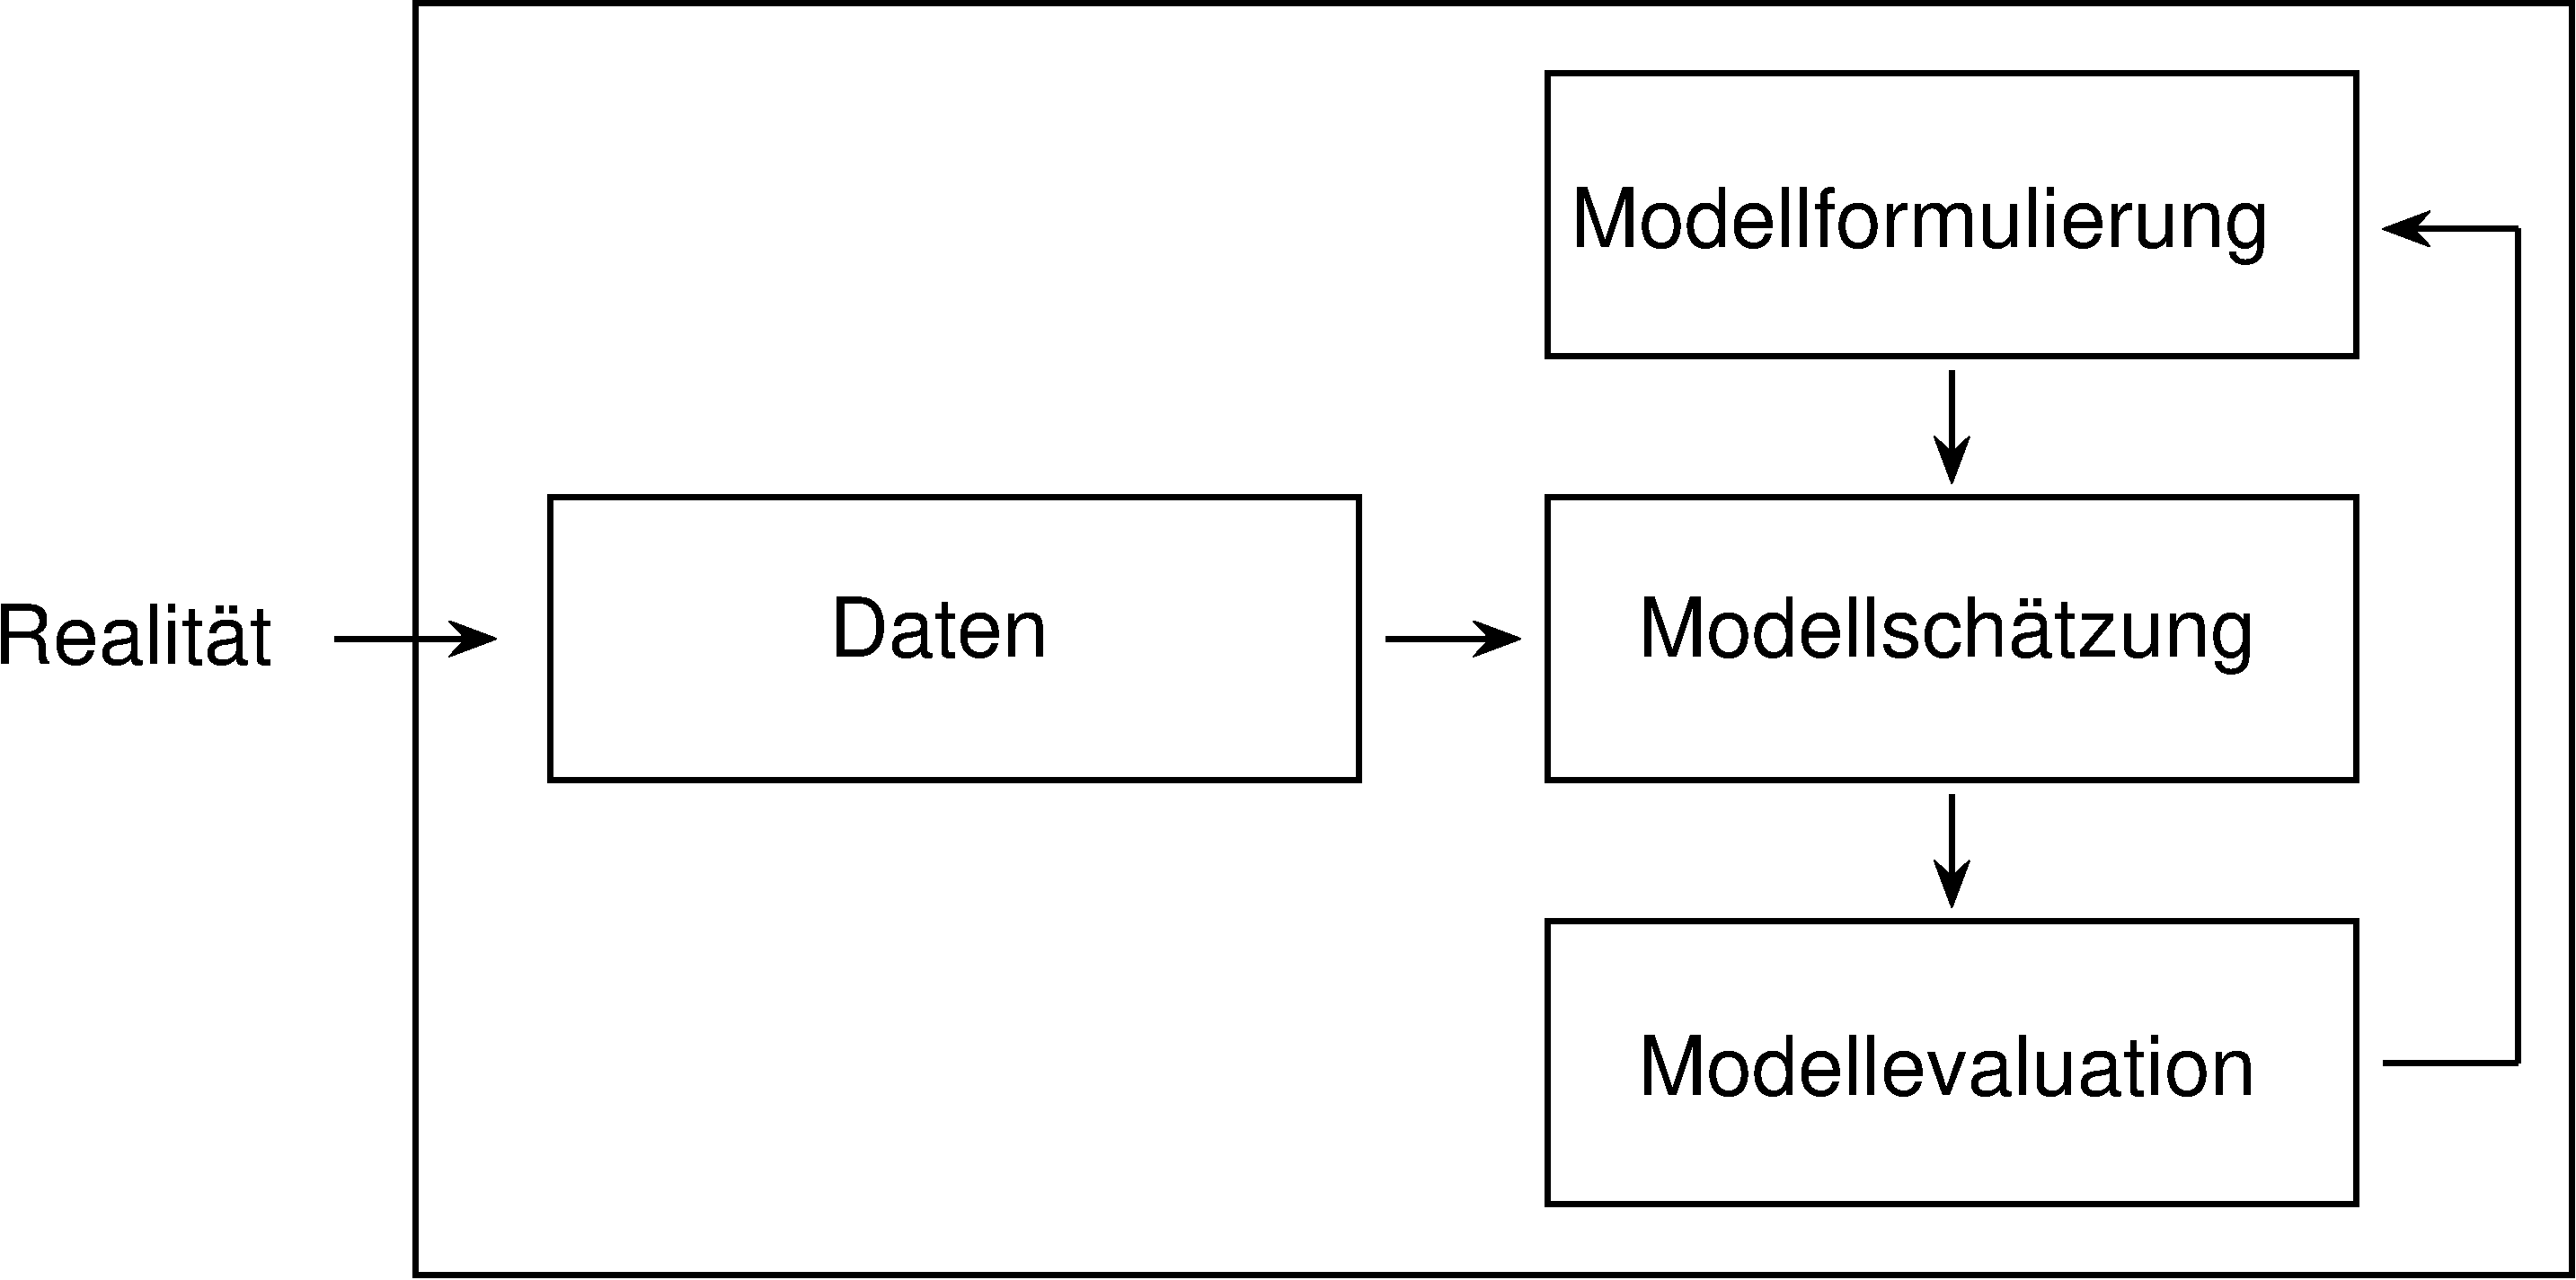
\includegraphics[width=0.9\linewidth]{6_Abbildungen/alm_6_wissenschaft} \end{center}
\end{frame}

\begin{frame}{}
\protect\hypertarget{section-3}{}
\vspace{1mm}
\normalsize

Modellformulierung \vspace{1mm} \small \begin{equation}
\upsilon = X\beta + \varepsilon, \varepsilon \sim N(0_n,\sigma^2I_n)
\end{equation} \vspace{5mm}

\normalsize

Modellschätzung \small \begin{equation}
\hat{\beta} = (X^TX)^{-1} X^T\upsilon,  \hat{\sigma}^2 = \frac{(\upsilon-X\hat{\beta})^T(\upsilon-X\hat{\beta})}{n-p}
\end{equation} \vspace{4mm}

\normalsize

Modellevaluation \small \begin{equation}
T = \frac{c^T\hat{\beta} - c^T\beta_0}{\sqrt{\hat{\sigma}^2c^T(X^TX)^{-1}c}},
F = \frac{(\hat{\varepsilon}_0^T\hat{\varepsilon}_0 - \hat{\varepsilon}^T\hat{\varepsilon})/p_1}{\hat{\varepsilon}^T\hat{\varepsilon}/(n-p)}
\end{equation}
\end{frame}

\begin{frame}{}
\protect\hypertarget{section-4}{}
Standardprobleme Frequentistischer Inferenz

\small
\vspace{2mm}

\noindent (1) Parameterschätzung

Ziel der Parameterschätzung ist es, einen möglichst guten Tipp für
wahre, aber unbekannte, Parameterwerte oder Funktionen dieser abzugeben,
typischerweise mithilfe von Daten.

\vspace{2mm}

\noindent (2) Konfidenzintervalle

Ziel der Bestimmung von Konfidenzintervallen ist es, basierend auf der
angenommenen Verteilung der Daten eine quantitative Aussage über die mit
Schätzwerten assoziierte Unsicherheit zu treffen.

\vspace{2mm}

\noindent (3) Hypothesentests

Ziel des Hypothesentestens ist es, basierend auf der angenommenen
Verteilung der Daten in einer möglichst zuverlässigen Form zu
entscheiden, ob ein wahrer, aber unbekannter Parameterwert in einer von
zwei sich gegenseitig ausschließenden Untermengen des Parameterraumes
liegt.
\end{frame}

\begin{frame}{}
\protect\hypertarget{section-5}{}
\center

\begin{center}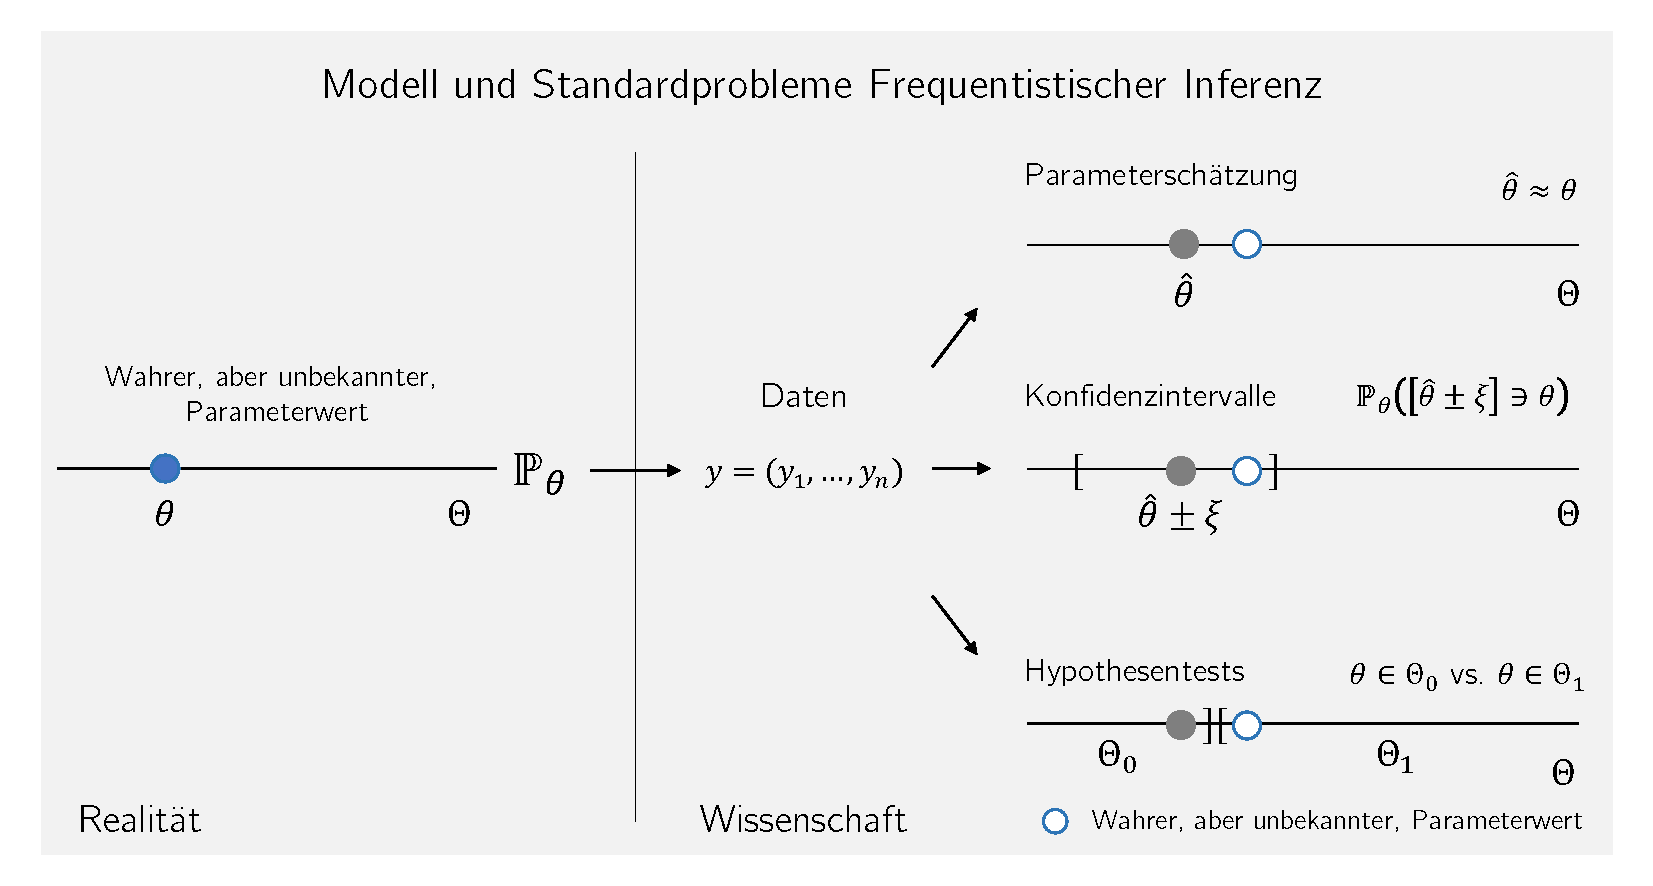
\includegraphics[width=1\linewidth]{6_Abbildungen/alm_6_frequentistische_inferenz} \end{center}
\center
\footnotesize

\(\theta := (\beta,\sigma^2)\),
\(\Theta := \mathbb{R}^p \times \mathbb{R}_{>0}\)
\(\mathbb{P}_\theta(\upsilon) := \mathbb{P}_{\beta,\sigma^2}(\upsilon)\)
mit WDF \(p_{\beta,\sigma^2}(y) := N(y;X\beta,\sigma^2I_n)\)
\end{frame}

\begin{frame}{}
\protect\hypertarget{section-6}{}
\small

Standardannahmen Frequentistischer Inferenz

\footnotesize
\setstretch{1.2}

Gegeben sei das Allgemeine Lineare Modell. Es wird angenommen, dass ein
vorliegender Datensatz eine der möglichen Realisierungen der Daten des
Modells ist. Aus Frequentistischer Sicht kann man unendlich oft
Datensätze basierend auf einem Modell generieren und zu jedem Datensatz
Schätzer oder Statistiken auswerten, z.B. den Betaparameterschätzer
\vspace{1mm}

\begin{itemize}
\item[] Datensatz (1) : $y^{(1)} = \left(y_1^{(1)}, y_2^{(1)}, ...,y_n^{(1)}\right)^T$  mit $\hat{\beta}^{(1)} = (X^TX)^{-1}X^Ty^{(1)}$
\item[] Datensatz (2) : $y^{(2)} = \left(y_1^{(2)}, y_2^{(2)}, ...,y_n^{(2)}\right)^T$  mit $\hat{\beta}^{(2)} = (X^TX)^{-1}X^Ty^{(2)}$
\item[] Datensatz (3) : $y^{(3)} = \left(y_1^{(3)}, y_2^{(3)}, ...,y_n^{(3)}\right)^T$  mit $\hat{\beta}^{(3)} = (X^TX)^{-1}X^Ty^{(3)}$
\item[] Datensatz (4) : $y^{(4)} = \left(y_1^{(4)}, y_2^{(4)}, ...,y_n^{(4)}\right)^T$  mit $\hat{\beta}^{(4)} = (X^TX)^{-1}X^Ty^{(4)}$
\item[] Datensatz (5) : $y^{(5)} = ...$
\end{itemize}

\vspace{1mm}

Um die Qualität statistischer Methoden zu beurteilen betrachtet die
Frequentistische Statistik die Wahrscheinlichkeitsverteilungen von
Schätzern und Statistiken unter Annahme der Datenverteilung. Was zum
Beispiel ist die Verteilung von \(\hat{\beta}^{(1)}\),
\(\hat{\beta}^{(2)}\), \(\hat{\beta}^{(3)}\), \(\hat{\beta}^{(4)}\),
\ldots{} also die Verteilung der Zufallsvariable
\(\hat{\beta} := (X^TX)^{-1}X^T\upsilon\)? Wenn eine statistische
Methode im Sinne der Frequentistischen Standardannahmen ``gut'' ist,
dann heißt das also, dass sie bei häufiger Anwendung ``im Mittel gut''
ist. Im Einzelfall, also im Normalfall nur eines vorliegenden
Datensatzes, kann sie auch ``schlecht'' sein.
\end{frame}

\begin{frame}{}
\protect\hypertarget{section-7}{}
\large
\setstretch{2.7}
\vfill

Allgemeine Theorie

Unabhängige und identisch normalverteilte Zufallsvariablen

Einfache lineare Regression

Frequentistische Schätzerverteilungen

Selbstkontrollfragen \vfill
\end{frame}

\begin{frame}{}
\protect\hypertarget{section-8}{}
\large
\setstretch{2.7}
\vfill

\textbf{Allgemeine Theorie}

Unabhängige und identisch normalverteilte Zufallsvariablen

Einfache lineare Regression

Frequentistische Schätzerverteilungen

Selbstkontrollfragen \vfill
\end{frame}

\begin{frame}{Allgemeine Theorie}
\protect\hypertarget{allgemeine-theorie}{}
\footnotesize
\begin{theorem}[Betaparameterschätzer]
\justifying
\normalfont
Es sei
\begin{equation}
\upsilon = X\beta + \varepsilon \mbox{ mit } \varepsilon \sim N(0_n,\sigma^2I_n)
\end{equation}
das ALM und es sei
\begin{equation}
\hat{\beta} := \left(X^TX\right)^{-1}X^T\upsilon.
\end{equation}
der \textit{Betaparameterschätzer}. Dann gilt, dass $\hat{\beta}$ die Summe der Abweichungsquadrate minimiert,
\begin{equation}
\hat{\beta} = \argmin_{\tilde{\beta}} (\upsilon-X\tilde{\beta})^T(\upsilon-X\tilde{\beta}),
\end{equation}
und dass $\hat{\beta}$ ein unverzerrter Maximum-Likelihood Schätzer von $\beta \in \mathbb{R}^p$ ist.
\end{theorem}

Bemerkungen

\begin{itemize}
\tightlist
\item
  Das Theorem gibt ein Formel an, um \(\beta\) anhand von Designmatrix
  und Daten zu schätzen.
\item
  Da \(\hat{\beta}\) die Summe der Abweichungsquadrate minimiert, heißt
  \(\hat{\beta}\) auch Kleinste-Quadrate (KQ) Schätzer.
\item
  Die \(\tilde{\beta}\) Notation des Maximierungarguments dient
  lediglich zur Abgrenzung vom w.a.u. \(\beta\).
\item
  Als ML Schätzer ist \(\hat{\beta}\) weiterhin konsistent, asymptotisch
  normalverteilt und asymptotisch effizient.
\item
  Wir sehen später, dass \(\hat{\beta}\) sogar normalverteilt ist.
\item
  Außerdem hat \(\hat{\beta}\) die ``kleinste Varianz'' in der Klasse
  der linearen unverzerrten Schätzer von \(\beta\).
\item
  Letztere Eigenschaft ist Kernaussage des
  \textit{Gauss-Markov Theorems}, auf das wir hier nicht näher eingehen
  wollen.
\item
  Für eine Diskussion und einen Beweis des Gauss-Markov Theorems siehe
  z.B. Searle (1971), Kapitel 3.
\end{itemize}
\end{frame}

\begin{frame}{Allgemeine Theorie}
\protect\hypertarget{allgemeine-theorie-1}{}
\footnotesize

\underline{Beweis}

\noindent (1) Wir zeigen in einem ersten Schritt, dass \(\hat{\beta}\)
die Summe der Abweichungsquadrate \begin{equation}
(\upsilon-X\tilde{\beta})^T(\upsilon-X\tilde{\beta})
\end{equation} minimiert. Dazu halten wir zunächst fest, dass
\begin{equation}
\hat{\beta} = (X^TX)^{-1}X^T\upsilon
\Leftrightarrow
X^TX\hat{\beta} = X^T\upsilon
\Leftrightarrow
X^T\upsilon - X^TX\hat{\beta} = 0_p
\Leftrightarrow
X^T(\upsilon -   X\hat{\beta}) = 0_p.
\end{equation} Weiterhin gilt dann auch, dass \begin{equation}
X^T(\upsilon -  X\hat{\beta}) = 0_p
\Leftrightarrow
\left(X^T(\upsilon -  X\hat{\beta})\right)^T = 0_p^T
\Leftrightarrow
(\upsilon -  X\hat{\beta})^TX = 0_p^T
\end{equation} Weiterhin halten wir ohne Beweis fest, dass für jede
Matrix \(X \in \mathbb{R}^{n \times p}\) gilt, dass \begin{equation}
z^TX^TXz \ge 0 \mbox{ für alle } z \in \mathbb{R}^p.
\end{equation} Wir betrachten nun die Summe der Abweichungsquadrate
\begin{equation}
(\upsilon -  X\tilde{\beta})^T(\upsilon -  X\tilde{\beta}).
\end{equation}
\end{frame}

\begin{frame}{Allgemeine Theorie}
\protect\hypertarget{allgemeine-theorie-2}{}
\footnotesize

\underline{Beweis (fortgeführt)}

Es ergibt sich dann \begin{align*}
\begin{split}
& (\upsilon-X\tilde{\beta})^T(\upsilon- X\tilde{\beta}) \\
& = (\upsilon-X\hat{\beta} + X\hat{\beta}- X\tilde{\beta})^T(\upsilon-X\hat{\beta} + X\hat{\beta} - X\tilde{\beta}) \\
& = ((\upsilon- X\hat{\beta}) + X(\hat{\beta}-\tilde{\beta}))^T((\upsilon-X\hat{\beta}) + X(\hat{\beta} -\tilde{\beta})) \\
& = (\upsilon-X\hat{\beta})^T(\upsilon- X\hat{\beta}) + (\upsilon -  X\hat{\beta})^T X(\hat{\beta} -\tilde{\beta})
     + (\hat{\beta}-\tilde{\beta})^TX^T(\upsilon- X\hat{\beta})
     + (\hat{\beta}-\tilde{\beta})^TX^TX(\hat{\beta} -\tilde{\beta}) \\
& = (\upsilon -  X\hat{\beta})^T(\upsilon -  X\hat{\beta})  +  0_p^T(\hat{\beta} -\tilde{\beta})
     + (\hat{\beta} -\tilde{\beta})^T0_p
     + (\hat{\beta} -\tilde{\beta})^TX^TX(\hat{\beta} -\tilde{\beta}) \\
&  = (\upsilon- X\hat{\beta})^T(\upsilon-X\hat{\beta}) + (\hat{\beta} -\tilde{\beta})^TX^TX(\hat{\beta} -\tilde{\beta}). \\
\end{split}
\end{align*} Auf der rechten Seite obiger Gleichung ist nur der zweite
Term von \(\tilde{\beta}\) abhängig. Da für diesen Term gilt, dass
\begin{equation}
(\hat{\beta} -\tilde{\beta})^TX^TX(\hat{\beta} -\tilde{\beta}) \ge 0
\end{equation} nimmt dieser Term genau dann seinen Minimalwert 0 an,
wenn \begin{equation}
(\hat{\beta} -\tilde{\beta}) = 0_p \Leftrightarrow \tilde{\beta} = \hat{\beta}.
\end{equation} Also gilt \begin{equation}
\hat{\beta} = \argmin_{\tilde{\beta}} (\upsilon -  X\tilde{\beta})^T(\upsilon -  X\tilde{\beta}).
\end{equation}
\end{frame}

\begin{frame}{Allgemeine Theorie}
\protect\hypertarget{allgemeine-theorie-3}{}
\footnotesize

\underline{Beweis (fortgeführt)}

\noindent (2) Um zu zeigen, dass \(\hat{\beta}\) ein Maximum Likelihood
Schätzer ist, betrachten wir für festes \(y \in \mathbb{R}^n\) und
festes \(\sigma^2 > 0\) die Log-Likelihood Funktion \begin{equation}
\ell : \mathbb{R}^p \to \mathbb{R}, \tilde{\beta} \mapsto \ln p_{\tilde{\beta}}(y) = \ln N(y;X\tilde{\beta}, \sigma^2I_n)
\end{equation} wobei gilt, dass \begin{align}
\begin{split}
\ln N(y;X\tilde{\beta}, \sigma^2I_n)
& = \ln\left((2\pi)^{-\frac{n}{2}}|\sigma^2I_n|^{-\frac{1}{2}}\exp\left(-\frac{1}{2\sigma^2}(\upsilon -  X\tilde{\beta})^T(\upsilon -  X\tilde{\beta})\right)\right) \\
& = -\frac{n}{2} \ln 2\pi - \frac{1}{2} \ln |\sigma^2I_n| - \frac{1}{2\sigma^2}(\upsilon -  X\tilde{\beta})^T(\upsilon -  X\tilde{\beta}).
\end{split}
\end{align} Dabei hängt allein der Term
\(-\frac{1}{2\sigma^2}(\upsilon - X\tilde{\beta})^T(\upsilon - X\tilde{\beta})\)
von \(\tilde{\beta}\) ab. Weil aber
\((\upsilon - X\tilde{\beta})^T(\upsilon - X\tilde{\beta}) \ge 0\), gilt
wird dieser Term aufgrund des negativen Vorzeichen maximal, wenn
\((\upsilon - X\tilde{\beta})^T(\upsilon - X\tilde{\beta})\) minimal
wird. Dies ist aber wie oben gezeigt genau für
\(\tilde{\beta} = \hat{\beta}\) der Fall.

\vspace{2mm}

\noindent (3) Die Unverzerrtheit von \(\hat{\beta}\) schließlich ergibt
sich aus \begin{align}
\begin{split}
\mathbb{E}(\hat{\beta})
= \mathbb{E}\left((X^TX)^{-1}X^T\upsilon\right)
= (X^TX)^{-1}X^T\mathbb{E}(\upsilon)
= (X^TX)^{-1}X^TX\beta
= \beta.
\end{split}
\end{align}
\end{frame}

\begin{frame}{Allgemeine Theorie}
\protect\hypertarget{allgemeine-theorie-4}{}
\footnotesize
\begin{definition}[Erklärte Daten, Residuenvektor, Residuen]
Es sei 
\begin{equation}
\upsilon = X\beta + \varepsilon \mbox{ mit } \varepsilon \sim N(0_n,\sigma^2I_n) 
\end{equation}
das Allgemeine Lineare Modell und es sei 
\begin{equation}
\hat{\beta} := (X^TX)^{-1}X^T\upsilon. 
\end{equation}
der Betaparameterschätzer. Dann heißt der Zufallsvektor
\begin{equation}
\hat{\upsilon} := X\hat{\beta} = X(X^TX)^{-1}X^T\upsilon
\end{equation}
die \textit{erklärten Daten}, der Zufallsvektor 
\begin{equation}
\hat{\varepsilon} := \upsilon - \hat{\upsilon} = \upsilon - X\hat{\beta}
\end{equation}
heißt \textit{Residuenvektor} und für $i = 1,...,n$ heißen die Komponenten dieses Zufallsvektors  
\begin{equation}
\hat{\varepsilon}_i := \upsilon_i - \hat{\upsilon}_i =  \upsilon_i - (X\hat{\beta})_i 
\end{equation}
die \textit{Residuen}. 
\end{definition}

Bemerkungen

\begin{itemize}
\tightlist
\item
  Die Begriffe sind analog zu den in Einheit (2) Korrelation
  eingeführten Begriffen.
\end{itemize}
\end{frame}

\begin{frame}{Allgemeine Theorie}
\protect\hypertarget{allgemeine-theorie-5}{}
\footnotesize
\setstretch{1.3}
\begin{theorem}[Varianzparameterschätzer]
\justifying
\normalfont
Es sei
\begin{equation}
\upsilon = X\beta + \varepsilon \mbox{ mit } \varepsilon \sim N(0_n,\sigma^2I_n)
\end{equation}
das ALM in generativer Form. Dann ist
\begin{equation}
\hat{\sigma}^2 := \frac{(\upsilon-X\hat{\beta})^T(\upsilon-X\hat{\beta})}{n - p}
\end{equation}
ein unverzerrter Schätzer von $\sigma^2 > 0$.
\end{theorem}
\vspace{-2mm}

\footnotesize

Bemerkungen

\begin{itemize}
\tightlist
\item
  Es handelt sich bei \(\hat{\sigma}^2\) \textit{nicht} um einen Maximum
  Likelihood Schätzer von \(\sigma^2\).
\item
  Für einen Beweis siehe z.B. Searle (1971), Kapitel 3 oder Rencher and
  Schaalje (2008), Kapitel 7.
\item
  Mit Definition des Residuenvektors und der Residuen bieten sich für
  \(\hat{\sigma}^2\) auch folgende Schreibweisen an: \begin{equation}
  \hat{\sigma}^2
  = \frac{\hat{\varepsilon}^T \hat{\varepsilon}}{n-p}
  = \frac{1}{n-p} \sum_{i=1}^n \hat{\varepsilon}_i^2
  = \frac{1}{n-p} \sum_{i=1}^n \left(\upsilon_i - (X\beta)_i \right)^2
  \end{equation}
\item
  \(\sigma^2\) wird also durch die eine skalierte Residualquadratsumme
  geschätzt.
\item
  Der Maximum Likelihood Schätzer des Varianzparameters ist
  \(\hat{\sigma}^2_{\tiny \mbox{ML}} := \frac{1}{n}\hat{\varepsilon}^T \hat{\varepsilon}\).
\end{itemize}
\end{frame}

\begin{frame}{}
\protect\hypertarget{section-9}{}
\large
\setstretch{2.7}
\vfill

\textbf{Allgemeine Theorie}

Unabhängige und identisch normalverteilte Zufallsvariablen

Einfache lineare Regression

Frequentistische Schätzerverteilungen

Selbstkontrollfragen \vfill
\end{frame}

\begin{frame}{Unabhängige und identisch normalverteilte
Zufallsvariablen}
\protect\hypertarget{unabhuxe4ngige-und-identisch-normalverteilte-zufallsvariablen}{}
\small

Wir betrachten das Szenario von \(n\) unabhängigen und identisch
normalverteilten Zufallsvariablen mit Erwartungswertparameter
\(\mu \in \mathbb{R}\) und Varianzparameter \(\sigma^2\),
\begin{equation}
\upsilon_i \sim N(\mu,\sigma^2) \mbox{ für } i = 1,...,n.
\end{equation} Dann gilt, wie unten gezeigt,
\begin{equation}\label{eq:iid_estimators}
\hat{\beta} = \frac{1}{n}\sum_{i=1}^n \upsilon_i =: \bar{\upsilon}
\mbox{ und }
\hat{\sigma}^2 = \frac{1}{n-1}\sum_{i=1}^n (\upsilon_i - \bar{\upsilon})^2 =: s^2_\upsilon.
\end{equation} In diesem Fall ist also der Betaparameterschätzer mit dem
Stichprobenmittel \(\bar{\upsilon}\) der \(\upsilon_1,...,\upsilon_n\)
und der Varianzparameterschätzer mit der Stichprobenvarianz
\(s_\upsilon^2\) der \(\upsilon_1,...,\upsilon_n\) identisch.
\end{frame}

\begin{frame}{Unabhängige und identisch normalverteilte
Zufallsvariablen}
\protect\hypertarget{unabhuxe4ngige-und-identisch-normalverteilte-zufallsvariablen-1}{}
\small

Für \(\hat{\beta}\) ergibt sich \begin{align*}
\begin{split}
\hat{\beta}
& = (X^TX)^{-1}X^T\upsilon
\\
& = \left(1_n^T 1_n\right)^{-1}1_n^T\upsilon
\\
& =
\left(
\begin{pmatrix}
1 & \cdots & 1\\
\end{pmatrix}
\begin{pmatrix}
1\\
\vdots \\
1\\
\end{pmatrix}
\right)^{-1}
\begin{pmatrix}
1 & \cdots & 1\\
\end{pmatrix}
\begin{pmatrix}
\upsilon_{1}\\
\vdots \\
\upsilon_{n}\\
\end{pmatrix}
\\
& = n^{-1}\sum_{i=1}^n \upsilon_i
\\
& =\frac{1}{n}\sum_{i=1}^n \upsilon_i
\\
& =: \bar{\upsilon}.
\end{split}
\end{align*}
\end{frame}

\begin{frame}{Unabhängige und identisch normalverteilte
Zufallsvariablen}
\protect\hypertarget{unabhuxe4ngige-und-identisch-normalverteilte-zufallsvariablen-2}{}
\small

Für \(\hat{\sigma}^2\) ergibt sich \begin{align*}
\begin{split}
\hat{\sigma}^2
& = \frac{1}{n-1}\left(\upsilon-X\hat{\beta}\right)^T\left(\upsilon-X\hat{\beta} \right)
\\
& = \frac{1}{n-1}\left(\upsilon-1_n\bar{\upsilon}\right)^T\left(\upsilon-1_n\bar{\upsilon}\right)
\\
& = \frac{1}{n-1}
\left(
\begin{pmatrix} \upsilon_1  \\  \vdots  \\  \upsilon_n  \end{pmatrix} -
\begin{pmatrix} 1           \\  \vdots  \\  1           \end{pmatrix}
\bar{\upsilon}
\right)^T
\left(
\begin{pmatrix} \upsilon_1  \\  \vdots  \\  \upsilon_n  \end{pmatrix} -
\begin{pmatrix} 1           \\  \vdots  \\  1           \end{pmatrix}
\bar{\upsilon}
\right)
\\
& =
\frac{1}{n-1}
\begin{pmatrix}
\upsilon_{1}-\bar{\upsilon}
& \cdots
& \upsilon_{n}-\bar{\upsilon}
\end{pmatrix}
\begin{pmatrix}
\upsilon_{1}-\bar{\upsilon} \\
\vdots \\
\upsilon_{n}-\bar{\upsilon} \\
\end{pmatrix}
\\
& = \frac{1}{n-1} \sum_{i=1}^n \left(\upsilon_i-\bar{\upsilon} \right)^2
\\
& =: s^2_\upsilon.
\end{split}
\end{align*}
\end{frame}

\begin{frame}[fragile]{Unabhängige und identisch normalverteilte
Zufallsvariablen}
\protect\hypertarget{unabhuxe4ngige-und-identisch-normalverteilte-zufallsvariablen-3}{}
Parameterschätzung \vspace{1mm}

\setstretch{1}
\tiny

\begin{Shaded}
\begin{Highlighting}[]
\CommentTok{\# Modellformulierung}
\FunctionTok{library}\NormalTok{(MASS)                                     }\CommentTok{\# Multivariate Normalverteilung}
\NormalTok{n          }\OtherTok{=} \DecValTok{12}                                   \CommentTok{\# Anzahl Datenpunkte}
\NormalTok{p          }\OtherTok{=} \DecValTok{1}                                    \CommentTok{\# Anzahl Betaparameter}
\NormalTok{X          }\OtherTok{=} \FunctionTok{matrix}\NormalTok{(}\FunctionTok{rep}\NormalTok{(}\DecValTok{1}\NormalTok{,n), }\AttributeTok{nrow =}\NormalTok{ n)           }\CommentTok{\# Designmatrix}
\NormalTok{I\_n        }\OtherTok{=} \FunctionTok{diag}\NormalTok{(n)                              }\CommentTok{\# n x n Einheitsmatrix}
\NormalTok{beta       }\OtherTok{=} \DecValTok{2}                                    \CommentTok{\# wahrer, aber unbekannter, Betaparameter}
\NormalTok{sigsqr     }\OtherTok{=} \DecValTok{1}                                    \CommentTok{\# wahrer, aber unbekannter, Varianzparameter}

\CommentTok{\# Datenrealisierung}
\NormalTok{y          }\OtherTok{=}  \FunctionTok{mvrnorm}\NormalTok{(}\DecValTok{1}\NormalTok{, X }\SpecialCharTok{\%*\%}\NormalTok{ beta, sigsqr}\SpecialCharTok{*}\NormalTok{I\_n)  }\CommentTok{\# eine Realisierung eines n{-}dimensionalen ZVs}

\CommentTok{\# Parameterschätzung}
\NormalTok{beta\_hat   }\OtherTok{=} \FunctionTok{solve}\NormalTok{(}\FunctionTok{t}\NormalTok{(X) }\SpecialCharTok{\%*\%}\NormalTok{ X) }\SpecialCharTok{\%*\%} \FunctionTok{t}\NormalTok{(X) }\SpecialCharTok{\%*\%}\NormalTok{ y     }\CommentTok{\# Betaparameterschätzer}
\NormalTok{eps\_hat    }\OtherTok{=}\NormalTok{ y }\SpecialCharTok{{-}}\NormalTok{ X }\SpecialCharTok{\%*\%}\NormalTok{ beta\_hat                   }\CommentTok{\# Residuenvektor}
\NormalTok{sigsqr\_hat }\OtherTok{=}\NormalTok{ (}\FunctionTok{t}\NormalTok{(eps\_hat) }\SpecialCharTok{\%*\%}\NormalTok{ eps\_hat) }\SpecialCharTok{/}\NormalTok{(n}\SpecialCharTok{{-}}\NormalTok{p)      }\CommentTok{\# Varianzparameterschätzer}

\CommentTok{\# Ausgabe}
\FunctionTok{cat}\NormalTok{(}\StringTok{"beta       : "}\NormalTok{, beta,}
    \StringTok{"}\SpecialCharTok{\textbackslash{}n}\StringTok{hat\{beta\}  : "}\NormalTok{, beta\_hat,}
    \StringTok{"}\SpecialCharTok{\textbackslash{}n}\StringTok{sigsqr     : "}\NormalTok{, sigsqr,}
    \StringTok{"}\SpecialCharTok{\textbackslash{}n}\StringTok{hat\{sigsqr\}: "}\NormalTok{, sigsqr\_hat)}
\end{Highlighting}
\end{Shaded}

\begin{verbatim}
> beta       :  2 
> hat{beta}  :  1.64 
> sigsqr     :  1 
> hat{sigsqr}:  1.12
\end{verbatim}
\end{frame}

\begin{frame}[fragile]{Unabhängige und identisch normalverteilte
Zufallsvariablen}
\protect\hypertarget{unabhuxe4ngige-und-identisch-normalverteilte-zufallsvariablen-4}{}
Simulation der Schätzerunverzerrtheit \vspace{1mm}

\setstretch{1}
\tiny

\begin{Shaded}
\begin{Highlighting}[]
\CommentTok{\# Modellformulierung}
\FunctionTok{library}\NormalTok{(MASS)                                        }\CommentTok{\# Multivariate Normalverteilung}
\NormalTok{n         }\OtherTok{=} \DecValTok{12}                                       \CommentTok{\# Anzahl Datenpunkte}
\NormalTok{p          }\OtherTok{=} \DecValTok{1}                                       \CommentTok{\# Anzahl Betaparameter}
\NormalTok{X          }\OtherTok{=} \FunctionTok{matrix}\NormalTok{(}\FunctionTok{rep}\NormalTok{(}\DecValTok{1}\NormalTok{,n), }\AttributeTok{nrow =}\NormalTok{ n)              }\CommentTok{\# Designmatrix}
\NormalTok{I\_n        }\OtherTok{=} \FunctionTok{diag}\NormalTok{(n)                                 }\CommentTok{\# n x n Einheitsmatrix}
\NormalTok{beta       }\OtherTok{=} \DecValTok{2}                                       \CommentTok{\# wahrer, aber unbekannter, Betaparameter}
\NormalTok{sigsqr     }\OtherTok{=} \DecValTok{1}                                       \CommentTok{\# wahrer, aber unbekannter, Varianzparameter}

\CommentTok{\# Frequentistische Simulation}
\NormalTok{nsim       }\OtherTok{=} \FloatTok{1e4}                                     \CommentTok{\# Anzahl Datenrealisierungen}
\NormalTok{beta\_hat   }\OtherTok{=} \FunctionTok{rep}\NormalTok{(}\ConstantTok{NaN}\NormalTok{,nsim)                           }\CommentTok{\# \textbackslash{}hat\{\textbackslash{}beta\} Realisierungsarray}
\NormalTok{sigsqr\_hat }\OtherTok{=} \FunctionTok{rep}\NormalTok{(}\ConstantTok{NaN}\NormalTok{,nsim)                           }\CommentTok{\# \textbackslash{}hat\{sigsqr\} Realisierungsarray}
\ControlFlowTok{for}\NormalTok{(i }\ControlFlowTok{in} \DecValTok{1}\SpecialCharTok{:}\NormalTok{nsim)\{                                    }\CommentTok{\# Simulationsiterationen}
\NormalTok{  y             }\OtherTok{=} \FunctionTok{mvrnorm}\NormalTok{(}\DecValTok{1}\NormalTok{, X }\SpecialCharTok{\%*\%}\NormalTok{ beta, sigsqr}\SpecialCharTok{*}\NormalTok{I\_n) }\CommentTok{\# Datenrealisierung}
\NormalTok{  beta\_hat[i]   }\OtherTok{=} \FunctionTok{solve}\NormalTok{(}\FunctionTok{t}\NormalTok{(X) }\SpecialCharTok{\%*\%}\NormalTok{ X) }\SpecialCharTok{\%*\%} \FunctionTok{t}\NormalTok{(X) }\SpecialCharTok{\%*\%}\NormalTok{ y   }\CommentTok{\# Betaparameterschätzer}
\NormalTok{  eps\_hat       }\OtherTok{=}\NormalTok{ y }\SpecialCharTok{{-}}\NormalTok{ X }\SpecialCharTok{\%*\%}\NormalTok{ beta\_hat[i]              }\CommentTok{\# Residuenvektor}
\NormalTok{  sigsqr\_hat[i] }\OtherTok{=}\NormalTok{ (}\FunctionTok{t}\NormalTok{(eps\_hat) }\SpecialCharTok{\%*\%}\NormalTok{ eps\_hat) }\SpecialCharTok{/}\NormalTok{(n}\SpecialCharTok{{-}}\NormalTok{p)    }\CommentTok{\# Varianzparameterschätzer}
\NormalTok{\}}

\CommentTok{\# Ausgabe}
\FunctionTok{cat}\NormalTok{(}\StringTok{"Wahrer, aber unbekannter, Betaparameter                  : "}\NormalTok{, beta,}
    \StringTok{"}\SpecialCharTok{\textbackslash{}n}\StringTok{Geschätzter Erwartungswert des Betaparameterschätzers    : "}\NormalTok{, }\FunctionTok{mean}\NormalTok{(beta\_hat),}
    \StringTok{"}\SpecialCharTok{\textbackslash{}n}\StringTok{Wahrer, aber unbekannter, Varianzparameter               : "}\NormalTok{, sigsqr,}
    \StringTok{"}\SpecialCharTok{\textbackslash{}n}\StringTok{Geschätzter Erwartungswert des Varianzparameterschätzers : "}\NormalTok{, }\FunctionTok{mean}\NormalTok{(sigsqr\_hat))}
\end{Highlighting}
\end{Shaded}

\begin{verbatim}
> Wahrer, aber unbekannter, Betaparameter                  :  2 
> Geschätzter Erwartungswert des Betaparameterschätzers    :  2 
> Wahrer, aber unbekannter, Varianzparameter               :  1 
> Geschätzter Erwartungswert des Varianzparameterschätzers :  0.998
\end{verbatim}
\end{frame}

\begin{frame}{}
\protect\hypertarget{section-10}{}
\large
\setstretch{2.7}
\vfill

Allgemeine Theorie

Unabhängige und identisch normalverteilte Zufallsvariablen

\textbf{Einfache lineare Regression}

Frequentistische Schätzerverteilungen

Selbstkontrollfragen \vfill
\end{frame}

\begin{frame}{Einfache lineare Regression}
\protect\hypertarget{einfache-lineare-regression}{}
\small

Wir betrachten das Modell der einfachen linearen Regression
\begin{equation}\label{eq:slr}
\upsilon_i = \beta_0 + \beta_1x_i + \varepsilon_i, \varepsilon_i \sim N(0,\sigma^2) \mbox{ für } i = 1,...,n,
\end{equation} Dann gilt wie unten gezeigt, dass
\begin{equation}\label{eq:slr_estimators}
\hat{\beta}
= \begin{pmatrix} \hat{\beta}_0 \\ \hat{\beta}_1 \end{pmatrix}
= \begin{pmatrix} \bar{\upsilon} - \frac{c_{x\upsilon}}{s_x^2}\bar{x} \\ \frac{c_{x\upsilon}}{s_x^2} \end{pmatrix}
\mbox{ und }
\hat{\sigma}^2 = \frac{1}{n-2}\sum_{i=1}^n (\upsilon_i - (\hat{\beta}_0 + \hat{\beta}_1x_i))^2
\end{equation} wobei

\begin{itemize}
\tightlist
\item
  \(\bar{x}\) und \(\bar{\upsilon}\) die Stichprobenmittel der
  \(x_1,...,x_n\) und \(\upsilon_1,...,\upsilon_n\), respektive,
  bezeichnen
\item
  \(c_{x\upsilon}\) die Stichprobenkovarianz der \(x_1, ...,x_n\) und
  \(\upsilon_1,...,\upsilon_n\) bezeichnet
\item
  \(s_x^2\) die Stichprobenvarianz der \(x_1,...,x_n\) bezeichnet.
\end{itemize}

Wie in (1) Regression sind die Bezeichnungen ``Stichproben''kovarianz
und ``Stichproben''varianz bezüglich der \(x_1,...,x_n\) hier lediglich
formal gemeint, da keine Annahme zugrundeliegt, dass die \(x_1,...,x_n\)
Realisierungen von Zufallsvariablen sind. Die \(x_1,...,x_n\) sind
vorgegebene Werte.
\end{frame}

\begin{frame}{Einfache lineare Regression}
\protect\hypertarget{einfache-lineare-regression-1}{}
\small

Wir halten fest, dass für eine parametrische Designmatrixspalte sich der
entsprechende Betaparameterschätzer aus der Stichprobenkovarianz der
respektiven Spalte mit den Daten geteilt durch die Stichprobenvarianz
der entsprechenden Spalte ergibt und somit einer ``standardisierten''
Stichprobenkovarianz entspricht. \vspace{2mm}

Ein Vergleich mit den Parametern der Ausgleichsgerade in (1) Regression
zeigt weiterhin die Identität der Betaparameterschätzerkomponenten
\(\hat{\beta}_0\) und \(\hat{\beta}_1\) mit den dort unter dem Kriterium
der Minimierung der quadrierten vertikalen Abweichungen hergeleiteten
Parametern. Dies überrascht nicht, da sowohl \(\hat{\beta}\) als auch
die Parameter der Ausgleichsgerade den Wert \begin{equation}
q(\tilde{\beta})
= \sum_{i=1}^n (\upsilon_i - (\tilde{\beta}_0 + \tilde{\beta}_1 x_i))^2
= (\upsilon -  X\tilde{\beta})^T(\upsilon -  X\tilde{\beta})
\end{equation} hinsichtlich \(\tilde{\beta}\) minimieren.
\end{frame}

\begin{frame}{Einfache lineare Regression}
\protect\hypertarget{einfache-lineare-regression-2}{}
\footnotesize

Um die Form des Betaparameterschätzers herzuleiten, halten wir zunächst
fest, dass \tiny \begin{align}
\begin{split}
\sum_{i=1}^n (x_i-\bar{x})(\upsilon_i-\bar{\upsilon})
& = \sum_{i=1}^n (x_i\upsilon_i - x_i\bar{\upsilon} - \bar{x}\upsilon_i + \bar{x}\bar{\upsilon}) \\
& = \sum_{i=1}^n x_i\upsilon_i
  - \sum_{i=1}^n x_i\bar{\upsilon}
  - \sum_{i=1}^n \bar{x}\upsilon_i
  + \sum_{i=1}^n \bar{x}\bar{\upsilon} \\
& = \sum_{i=1}^n x_i\upsilon_i
  - \bar{\upsilon} \sum_{i=1}^n x_i
  - \bar{x}\sum_{i=1}^n \upsilon_i
  + n \bar{x}\bar{\upsilon} \\
& = \sum_{i=1}^n x_i\upsilon_i
  - \bar{\upsilon}n\bar{x}
  - \bar{x}n\bar{\upsilon}
  + n\bar{x}\bar{\upsilon} \\
  & = \sum_{i=1}^n x_i\upsilon_i
  - n\bar{x}\bar{\upsilon}
  - n\bar{x}\bar{\upsilon}
  + n\bar{x}\bar{\upsilon} \\
& = \sum_{i=1}^n x_i \upsilon_i  - n \bar{x}\bar{\upsilon},
\end{split}
\end{align}
\end{frame}

\begin{frame}{Einfache lineare Regression}
\protect\hypertarget{einfache-lineare-regression-3}{}
\footnotesize

Weiterhin halten wir fest, dass \tiny \begin{align}
\begin{split}
\sum_{i=1}^n (x_i - \bar{x})^2
& = \sum_{i=1}^n (x_i^2 - 2x_i\bar{x}  + \bar{x}^2) \\
& = \sum_{i=1}^n x_i^2 - \sum_{i=1}^n 2x_i\bar{x}  + \sum_{i=1}^n \bar{x}^2 \\
& = \sum_{i=1}^n x_i^2 - 2\bar{x}\sum_{i=1}^n x_i  + n\bar{x}^2 \\
& = \sum_{i=1}^n x_i^2 - 2\bar{x}n\bar{x}  + n\bar{x}^2 \\
& = \sum_{i=1}^n x_i^2 - 2n\bar{x}^2 + n\bar{x}^2 \\
& = \sum_{i=1}^n x_i^2 - n\bar{x}^2. 
\end{split}
\end{align}
\end{frame}

\begin{frame}{Einfache lineare Regression}
\protect\hypertarget{einfache-lineare-regression-4}{}
\footnotesize

Aus der Definition von \(\hat{\beta}\) ergibt sich \begin{align}
\begin{split}
\hat{\beta}
& = (X^T X)^{-1}X^T\upsilon \\
& =
\left(
\begin{pmatrix}
1   & \cdots & 1 \\
x_1 & \cdots & x_n
\end{pmatrix}
\begin{pmatrix}
1       & x_1       \\
\vdots  & \vdots    \\
1       & x_n
\end{pmatrix}
\right)^{-1}
\begin{pmatrix}
1   & \cdots & 1 \\
x_1 & \cdots & x_n
\end{pmatrix}
\begin{pmatrix}
\upsilon_1     \\
\vdots  \\
\upsilon_n
\end{pmatrix} \\
& =
\begin{pmatrix}
n                   & \sum_{i=1}^n x_i \\
\sum_{i=1}^n x_i    & \sum_{i=1}^n x_i^2\\
\end{pmatrix}^{-1}
\begin{pmatrix}
\sum_{i=1}^n \upsilon_i    \\
\sum_{i=1}^n x_i \upsilon_i    \\
\end{pmatrix}
\\
& =
\begin{pmatrix}
n           &  n\bar{x} \\
n\bar{x}    & \sum_{i=1}^n x_i^2\\
\end{pmatrix}^{-1}
\begin{pmatrix}
n\bar{\upsilon}    \\
\sum_{i=1}^n x_i \upsilon_i    \\
\end{pmatrix}.
\end{split}
\end{align}

Die Inverse von \(X^T X\) ist gegeben durch \begin{equation}
\frac{1}{s_x^2}
\begin{pmatrix}
  \frac{s_x^2}{n} + \bar{x}^2
& -\bar{x}
\\
  -\bar{x}
&  1
\end{pmatrix},
\end{equation}
\end{frame}

\begin{frame}{Einfache lineare Regression}
\protect\hypertarget{einfache-lineare-regression-5}{}
\footnotesize

weil \begin{align}
\begin{split}
& \frac{1}{s_x^2}
\begin{pmatrix}
  \frac{s_x^2}{n} + \bar{x}^2
& -\bar{x}
\\
  -\bar{x}
&  1
\end{pmatrix}
\begin{pmatrix}
n           &  n\bar{x} \\
n\bar{x}    & \sum_{i=1}^n x_i^2\\
\end{pmatrix}
\\
& =
\frac{1}{s_x^2}
\begin{pmatrix}
\frac{ns_x^2}{n} + n\bar{x}^2 - n \bar{x}^2
& \frac{s_x^2n\bar{x}}{n} +n\bar{x}^2\bar{x} - \bar{x}\sum_{i=1}^n x_i^2
\\
-\bar{x}n + n \bar{x}
& - n\bar{x}^2 + \sum_{i=1}^n x_i^2
\end{pmatrix} \\
& =
\frac{1}{s_x^2}
\begin{pmatrix}
s_x^2
& s_x^2\bar{x} -\bar{x} \left(\sum_{i=1}^n x_i^2 - n\bar{x}^2\right)
\\
0
& \sum_{i=1}^n x_i^2 - n\bar{x}^2
\end{pmatrix}
\\
& =
\frac{1}{s_x^2}
\begin{pmatrix}
s_x^2
& s_x^2\bar{x} - \bar{x} s_x^2
\\
0
& s_x^2
\end{pmatrix}
\\
& =
\frac{1}{s_x^2}
\begin{pmatrix}
s_x^2
& 0
\\
0
& s_x^2
\end{pmatrix}
\\
& =
\begin{pmatrix}
1 & 0 \\ 0 & 1
\end{pmatrix}.
\end{split}
\end{align}
\end{frame}

\begin{frame}{Einfache lineare Regression}
\protect\hypertarget{einfache-lineare-regression-6}{}
\footnotesize

Es ergibt sich also \begin{align}
\renewcommand{\arraystretch}{1.2}
\begin{split}
\hat{\beta}
= \begin{pmatrix}
  \frac{1}{n} + \frac{\bar{x}^2}{s_x^2}
& -\frac{\bar{x}}{s_x^2}
\\
  -\frac{\bar{x}}{s_x^2}
&  \frac{1}{s_x^2}
\end{pmatrix}
\begin{pmatrix}
n\bar{\upsilon}    \\
\sum_{i=1}^n x_i \upsilon_i    \\
\end{pmatrix}
& = \begin{pmatrix}
\left(\frac{1}{n} + \frac{\bar{x}^2}{s_x^2}\right)n\bar{\upsilon} - \frac{\bar{x}\sum_{i=1}^n x_i\upsilon_i}{s_x^2}   \\
\frac{\sum_{i=1}^n x_i \upsilon_i }{s_x^2} - \frac{n\bar{x}\bar{\upsilon}}{s_x^2} \\
\end{pmatrix}
\\
&
=
\begin{pmatrix}
\frac{n\bar{\upsilon}}{n} + \frac{\bar{x}^2n\bar{\upsilon}}{s_x^2}- \frac{\bar{x}\sum_{i=1}^n x_i\upsilon_i}{s_x^2}
\\
\frac{\sum_{i=1}^n x_i \upsilon_i - n\bar{x}\bar{\upsilon}}{s_x^2}    \\
\end{pmatrix}
\\
& =
\begin{pmatrix}
\bar{\upsilon} + \frac{\bar{x}n\bar{x}\bar{\upsilon} - \bar{x}\sum_{i=1}^n x_i\upsilon_i}{s_x^2}
\\
\frac{\sum_{i=1}^n x_i \upsilon_i - n\bar{x}\bar{\upsilon}}{s_x^2}    \\
\end{pmatrix}
\\
& =
\begin{pmatrix}
\bar{\upsilon} - \frac{\sum_{i=1}^n x_i\upsilon_i - n\bar{x}\bar{\upsilon}}{s_x^2}\bar{x}
\\
\frac{\sum_{i=1}^n x_i \upsilon_i - n\bar{x}\bar{\upsilon}}{s_x^2}
\end{pmatrix}
\\
& =
\begin{pmatrix}
\bar{\upsilon} - \frac{c_{x\upsilon}}{s_x^2}\bar{x}
\\
\frac{c_{x\upsilon}}{s_x^2}
\end{pmatrix}.
\end{split}
\end{align}
\end{frame}

\begin{frame}[fragile]{Einfache lineare Regression}
\protect\hypertarget{einfache-lineare-regression-7}{}
\vspace{1mm}

Parameterschätzung \vspace{2mm} \setstretch{1} \tiny

\begin{Shaded}
\begin{Highlighting}[]
\CommentTok{\# Modellformulierung}
\FunctionTok{library}\NormalTok{(MASS)                                    }\CommentTok{\# Multivariate Normalverteilung}
\NormalTok{n          }\OtherTok{=} \DecValTok{10}                                  \CommentTok{\# Anzahl Datenpunkte}
\NormalTok{p          }\OtherTok{=} \DecValTok{2}                                   \CommentTok{\# Anzahl Betaparameter}
\NormalTok{x          }\OtherTok{=} \DecValTok{1}\SpecialCharTok{:}\NormalTok{n                                 }\CommentTok{\# Prädiktorwerte}
\NormalTok{X          }\OtherTok{=} \FunctionTok{matrix}\NormalTok{(}\FunctionTok{c}\NormalTok{(}\FunctionTok{rep}\NormalTok{(}\DecValTok{1}\NormalTok{,n),x), }\AttributeTok{nrow =}\NormalTok{ n)     }\CommentTok{\# Designmatrix}
\NormalTok{I\_n        }\OtherTok{=} \FunctionTok{diag}\NormalTok{(n)                             }\CommentTok{\# n x n Einheitsmatrix}
\NormalTok{beta       }\OtherTok{=} \FunctionTok{matrix}\NormalTok{(}\FunctionTok{c}\NormalTok{(}\DecValTok{0}\NormalTok{,}\DecValTok{1}\NormalTok{), }\AttributeTok{nrow =}\NormalTok{ p)            }\CommentTok{\# wahrer, aber unbekannter, Betaparameter}
\NormalTok{sigsqr     }\OtherTok{=} \DecValTok{1}                                   \CommentTok{\# wahrer, aber unbekannter, Varianzparameter}

\CommentTok{\# Datenrealisierung}
\NormalTok{y          }\OtherTok{=} \FunctionTok{mvrnorm}\NormalTok{(}\DecValTok{1}\NormalTok{, X }\SpecialCharTok{\%*\%}\NormalTok{ beta, sigsqr}\SpecialCharTok{*}\NormalTok{I\_n)  }\CommentTok{\# eine Realisierung eines n{-}dimensionalen ZVs}

\CommentTok{\# Parameterschätzung}
\NormalTok{beta\_hat   }\OtherTok{=} \FunctionTok{solve}\NormalTok{(}\FunctionTok{t}\NormalTok{(X) }\SpecialCharTok{\%*\%}\NormalTok{ X) }\SpecialCharTok{\%*\%} \FunctionTok{t}\NormalTok{(X) }\SpecialCharTok{\%*\%}\NormalTok{ y    }\CommentTok{\# Betaparameterschätzer}
\NormalTok{eps\_hat    }\OtherTok{=}\NormalTok{ y }\SpecialCharTok{{-}}\NormalTok{ X }\SpecialCharTok{\%*\%}\NormalTok{ beta\_hat                  }\CommentTok{\# Residuenvektor}
\NormalTok{sigsqr\_hat }\OtherTok{=}\NormalTok{ (}\FunctionTok{t}\NormalTok{(eps\_hat) }\SpecialCharTok{\%*\%}\NormalTok{ eps\_hat) }\SpecialCharTok{/}\NormalTok{(n}\SpecialCharTok{{-}}\NormalTok{p)     }\CommentTok{\# Varianzparameterschätzer}

\CommentTok{\# Ausgabe}
\FunctionTok{cat}\NormalTok{(}\StringTok{"beta       : "}\NormalTok{, beta,}
    \StringTok{"}\SpecialCharTok{\textbackslash{}n}\StringTok{hat\{beta\}  : "}\NormalTok{, beta\_hat,}
    \StringTok{"}\SpecialCharTok{\textbackslash{}n}\StringTok{sigsqr     : "}\NormalTok{, sigsqr,}
    \StringTok{"}\SpecialCharTok{\textbackslash{}n}\StringTok{hat\{sigsqr\}: "}\NormalTok{, sigsqr\_hat)}
\end{Highlighting}
\end{Shaded}

\begin{verbatim}
> beta       :  0 1 
> hat{beta}  :  -1.04 1.07 
> sigsqr     :  1 
> hat{sigsqr}:  0.337
\end{verbatim}
\end{frame}

\begin{frame}[fragile]{Einfache lineare Regression}
\protect\hypertarget{einfache-lineare-regression-8}{}
\vspace{1mm}

Simulation der Schätzerunverzerrtheit \vspace{2mm}

\setstretch{1}
\tiny

\begin{Shaded}
\begin{Highlighting}[]
\CommentTok{\# Modellformulierung}
\FunctionTok{library}\NormalTok{(MASS)                                        }\CommentTok{\# Multivariate Normalverteilung}
\NormalTok{n          }\OtherTok{=} \DecValTok{10}                                      \CommentTok{\# Anzahl Datenpunkte}
\NormalTok{p          }\OtherTok{=} \DecValTok{2}                                       \CommentTok{\# Anzahl Betaparameter}
\NormalTok{x          }\OtherTok{=} \DecValTok{1}\SpecialCharTok{:}\NormalTok{n                                     }\CommentTok{\# Prädiktorwerte}
\NormalTok{X          }\OtherTok{=} \FunctionTok{matrix}\NormalTok{(}\FunctionTok{c}\NormalTok{(}\FunctionTok{rep}\NormalTok{(}\DecValTok{1}\NormalTok{,n),x), }\AttributeTok{nrow =}\NormalTok{ n)         }\CommentTok{\# Designmatrix}
\NormalTok{I\_n        }\OtherTok{=} \FunctionTok{diag}\NormalTok{(n)                                 }\CommentTok{\# n x n Einheitsmatrix}
\NormalTok{beta       }\OtherTok{=} \FunctionTok{matrix}\NormalTok{(}\FunctionTok{c}\NormalTok{(}\DecValTok{0}\NormalTok{,}\DecValTok{1}\NormalTok{), }\AttributeTok{nrow =}\NormalTok{ p)                }\CommentTok{\# wahrer, aber unbekannter, Betaparameter}
\NormalTok{sigsqr     }\OtherTok{=} \DecValTok{1}                                       \CommentTok{\# wahrer, aber unbekannter, Varianzparameter}

\CommentTok{\# Frequentistische Simulation}
\NormalTok{nsim       }\OtherTok{=} \FloatTok{1e4}                                     \CommentTok{\# Anzahl Realisierungen des n{-}dimensionalen ZVs}
\NormalTok{beta\_hat   }\OtherTok{=} \FunctionTok{matrix}\NormalTok{(}\FunctionTok{rep}\NormalTok{(}\ConstantTok{NaN}\NormalTok{,p}\SpecialCharTok{*}\NormalTok{nsim), }\AttributeTok{nrow =}\NormalTok{ p)       }\CommentTok{\# \textbackslash{}hat\{\textbackslash{}beta\} Realisierungsarray}
\NormalTok{sigsqr\_hat }\OtherTok{=} \FunctionTok{rep}\NormalTok{(}\ConstantTok{NaN}\NormalTok{,nsim)                           }\CommentTok{\# \textbackslash{}hat\{sigsqr\} Realisierungsarray}
\ControlFlowTok{for}\NormalTok{(i }\ControlFlowTok{in} \DecValTok{1}\SpecialCharTok{:}\NormalTok{nsim)\{                                    }\CommentTok{\# Simulationsiterationen}
\NormalTok{  y             }\OtherTok{=} \FunctionTok{mvrnorm}\NormalTok{(}\DecValTok{1}\NormalTok{, X }\SpecialCharTok{\%*\%}\NormalTok{ beta, sigsqr}\SpecialCharTok{*}\NormalTok{I\_n) }\CommentTok{\# Datenrealisierung}
\NormalTok{  beta\_hat[,i]  }\OtherTok{=} \FunctionTok{solve}\NormalTok{(}\FunctionTok{t}\NormalTok{(X) }\SpecialCharTok{\%*\%}\NormalTok{ X) }\SpecialCharTok{\%*\%} \FunctionTok{t}\NormalTok{(X) }\SpecialCharTok{\%*\%}\NormalTok{ y   }\CommentTok{\# Betaparameterschätzer}
\NormalTok{  eps\_hat       }\OtherTok{=}\NormalTok{ y }\SpecialCharTok{{-}}\NormalTok{ X }\SpecialCharTok{\%*\%}\NormalTok{ beta\_hat[,i]             }\CommentTok{\# Residuenvektor}
\NormalTok{  sigsqr\_hat[i] }\OtherTok{=}\NormalTok{ (}\FunctionTok{t}\NormalTok{(eps\_hat) }\SpecialCharTok{\%*\%}\NormalTok{ eps\_hat) }\SpecialCharTok{/}\NormalTok{(n}\SpecialCharTok{{-}}\NormalTok{p)    }\CommentTok{\# Varianzparameterschätzer}
\NormalTok{\}}

\CommentTok{\# Ausgabe}
\FunctionTok{cat}\NormalTok{(}\StringTok{"Wahrer, aber unbekannter, Betaparameter                  : "}\NormalTok{, beta,}
    \StringTok{"}\SpecialCharTok{\textbackslash{}n}\StringTok{Geschätzter Erwartungswert des Betaparameterschätzers    : "}\NormalTok{, }\FunctionTok{rowMeans}\NormalTok{(beta\_hat),}
    \StringTok{"}\SpecialCharTok{\textbackslash{}n}\StringTok{Wahrer, aber unbekannter, Varianzparameter               : "}\NormalTok{, sigsqr,}
    \StringTok{"}\SpecialCharTok{\textbackslash{}n}\StringTok{Geschätzter Erwartungswert des Varianzparameterschätzers : "}\NormalTok{, }\FunctionTok{mean}\NormalTok{(sigsqr\_hat))}
\end{Highlighting}
\end{Shaded}

\begin{verbatim}
> Wahrer, aber unbekannter, Betaparameter                  :  0 1 
> Geschätzter Erwartungswert des Betaparameterschätzers    :  -0.00191 1 
> Wahrer, aber unbekannter, Varianzparameter               :  1 
> Geschätzter Erwartungswert des Varianzparameterschätzers :  1.01
\end{verbatim}
\end{frame}

\begin{frame}{}
\protect\hypertarget{section-11}{}
\large
\setstretch{2.7}
\vfill

Allgemeine Theorie

Unabhängige und identisch normalverteilte Zufallsvariablen

Einfache lineare Regression

\textbf{Frequentistische Schätzerverteilungen}

Selbstkontrollfragen \vfill
\end{frame}

\begin{frame}{Frequentistische Schätzerverteilungen}
\protect\hypertarget{frequentistische-schuxe4tzerverteilungen}{}
\footnotesize
\begin{theorem}[Frequentistische Verteilung des Betaparameterschätzers]
\justifying
\normalfont
Es sei
\begin{equation}
\upsilon = X\beta + \varepsilon \mbox{ mit } \varepsilon \sim N(0_n,\sigma^2I_n)
\end{equation}
das ALM. Weiterhin sei
\begin{equation}
\hat{\beta} := \left(X^TX\right)^{-1}X^T\upsilon
\end{equation}
der Betaparameterschätzer. Dann gilt
\begin{equation}
\hat{\beta} \sim N\left(\beta,\sigma^2(X^T X)^{-1}\right).
\end{equation}
\end{theorem}

Bemerkungen

\begin{itemize}
\tightlist
\item
  \justifying Es gilt also wie bereits gesehen
  \(\mathbb{E}(\hat{\beta}) = \beta\) und außerdem
  \(\mathbb{C}(\hat{\beta}) = \sigma^2(X^TX)^{-1}\).
\item
  Die Varianzen der Komponenten von \(\hat{\beta}\) sind die
  Diagonalelemente von \(\mathbb{C}(\hat{\beta})\), also
  \begin{equation}
  \mathbb{V}(\hat{\beta}_i) = (\sigma^2(X^TX)^{-1})_{ii} \mbox{ für } i = 1,...p.
  \end{equation}
\item
  Die Streuung von \(\hat{\beta}\) hängt von \(\sigma^2\) und der
  Designmatrix \(X\) ab. \(\sigma^2\) ist ein experimentell nicht zu
  beinflussender wahrer, aber unbekannter, Parameter \(X\) dagegen kann
  so gewählt werden, um zum Beispiel die Diagonalelemente von
  \(\mathbb{C}(\hat{\beta})\) bei festem \(\sigma^2\) zu minimieren.
\end{itemize}
\end{frame}

\begin{frame}{Frequentistische Schätzerverteilungen}
\protect\hypertarget{frequentistische-schuxe4tzerverteilungen-1}{}
\footnotesize

\underline{Beweis}

Das Theorem folgt direkt mit dem Theorem zur linearen Transformation von
multivariaten Normalverteilung aus Einheit (4) Normalverteilungen.
Speziell gilt hier: \begin{equation}
\hat{\beta}
\sim
N\left(
(X^{T}X)^{-1}X^{T}X\beta,
(X^{T}X)^{-1}X^{T}(\sigma^{2}I_{n})((X^{T}X)^{-1}X^{T})^{T}
\right).
\end{equation} Der Erwartungswertparameter vereinfacht sich dann zu
\begin{equation}
(X^{T}X)^{-1}X^{T}X\beta = \beta.
\end{equation} Der Kovarianzmatrixparamter vereinfacht sich wie folgt
\begin{align}
\begin{split}
(X^{T}X)^{-1}X^{T}(\sigma^{2}I_{n})((X^{T}X)^{-1}X^{T})^{T}
&  =(X^{T}X)^{-1}X^{T}(\sigma^{2}I_{n})X(X^{T}X)^{-1}               \\
&  =\sigma^{2}(X^{T}X)^{-1}X^{T}X(X^{T}X)^{-1}                      \\
&  =\sigma^{2}(X^{T}X)^{-1}.
\end{split}
\end{align} Dabei folgt hier die erste Gleichung aus der Tatsache, dass
sowohl \(X^{T}X\) als auch ihre Inverse \((X^{T}X)^{-1}\) symmetrische
Matrizen sind.

Damit gilt dann insgesamt aber sofort \begin{equation}
\hat{\beta} \sim N\left(\beta,\sigma^2(X^T X)^{-1}\right).
\end{equation}
\end{frame}

\begin{frame}{Frequentistische Schätzerverteilungen}
\protect\hypertarget{frequentistische-schuxe4tzerverteilungen-2}{}
Beispiel (1) Unabhängige und identisch normalverteilte Zufallsvariablen
\vspace{1mm}

\small

Es sei \begin{equation}
\upsilon \sim N(X\beta,\sigma^2 I_n)
\mbox{ mit }
X := 1_n \in \mathbb{R}^{n\times 1},
\beta := \mu \in \mathbb{R}
\mbox{ und } \sigma^2 > 0.
\end{equation} das ALM Szenario unabhängiger und identisch
normalverteilter Zufallsvariablen. Wir haben bereits gesehen, dass
\(\hat{\beta} = \bar{\upsilon}\). Das Theorem zur Frequentistischen
Verteilung des Betaparameterschätzers impliziert damit \begin{equation}
\bar{\upsilon} \sim N\left(\mu, \frac{\sigma^2}{n}\right).
\end{equation} Das Stichprobenmittel von \(n\) unabhängigen und
identisch normalverteilten Zufallsvariablen mit Erwartungswertparameter
\(\mu\) und Varianzparameter \(\sigma^2\) ist also normalverteilt mit
Erwartungswertparameter \(\mu\) und Varianzparameter \(\sigma^2/n\). Wir
haben diese Tatsache bereits in Einheit (8) Transformationen der
Normalverteilungen in Wahrscheinlichkeitstheorie und Frequentistische
Inferenz unter dem Begriff der Mittelwertstransformation kennengelernt.
\end{frame}

\begin{frame}[fragile]{Frequentistische Schätzerverteilungen}
\protect\hypertarget{frequentistische-schuxe4tzerverteilungen-3}{}
Beispiel (1) Unabhängige und identisch normalverteilte Zufallsvariablen
\vspace{2mm}

\footnotesize

\begin{Shaded}
\begin{Highlighting}[]
\CommentTok{\# Modellformulierung}
\FunctionTok{library}\NormalTok{(MASS)                                      }\CommentTok{\# Multivariate Normalverteilung  }
\NormalTok{n        }\OtherTok{=} \DecValTok{12}                                      \CommentTok{\# Anzahl von Datenpunkten}
\NormalTok{p        }\OtherTok{=} \DecValTok{1}                                       \CommentTok{\# Anzahl von Betparametern}
\NormalTok{X        }\OtherTok{=} \FunctionTok{matrix}\NormalTok{(}\FunctionTok{rep}\NormalTok{(}\DecValTok{1}\NormalTok{,n), }\AttributeTok{nrow =}\NormalTok{ n)              }\CommentTok{\# Designmatrix}
\NormalTok{I\_n      }\OtherTok{=} \FunctionTok{diag}\NormalTok{(n)                                 }\CommentTok{\# n x n Einheitsmatrix}
\NormalTok{beta     }\OtherTok{=} \DecValTok{2}                                       \CommentTok{\# wahrer, aber unbekannter, Betaparameter}
\NormalTok{sigsqr   }\OtherTok{=} \DecValTok{1}                                       \CommentTok{\# wahrer, aber unbekannter, Varianzparameter}

\CommentTok{\# Frequentistische Simulation}
\NormalTok{nsim     }\OtherTok{=} \FloatTok{1e4}                                     \CommentTok{\# Anzahl Realisierungen des n{-}dimensionalen ZVs}
\NormalTok{beta\_hat }\OtherTok{=} \FunctionTok{rep}\NormalTok{(}\ConstantTok{NaN}\NormalTok{,nsim)                           }\CommentTok{\# \textbackslash{}hat\{\textbackslash{}beta\} Realisierungsarray}
\ControlFlowTok{for}\NormalTok{(i }\ControlFlowTok{in} \DecValTok{1}\SpecialCharTok{:}\NormalTok{nsim)\{}
\NormalTok{  y           }\OtherTok{=} \FunctionTok{mvrnorm}\NormalTok{(}\DecValTok{1}\NormalTok{, X }\SpecialCharTok{\%*\%}\NormalTok{ beta, sigsqr}\SpecialCharTok{*}\NormalTok{I\_n) }\CommentTok{\# eine Realisierung eines n{-}dimensionalen ZVs}
\NormalTok{  beta\_hat[i] }\OtherTok{=} \FunctionTok{solve}\NormalTok{(}\FunctionTok{t}\NormalTok{(X) }\SpecialCharTok{\%*\%}\NormalTok{ X) }\SpecialCharTok{\%*\%} \FunctionTok{t}\NormalTok{(X) }\SpecialCharTok{\%*\%}\NormalTok{ y   }\CommentTok{\# \textbackslash{}hat\{\textbackslash{}beta\} = (X\^{}T)X\^{}\{{-}1\}X\^{}T\textbackslash{}upsilon}
\NormalTok{\}}
\end{Highlighting}
\end{Shaded}
\end{frame}

\begin{frame}{Schätzerverteilungen}
\protect\hypertarget{schuxe4tzerverteilungen}{}
Beispiel (1) Unabhängige und identisch normalverteilte Zufallsvariablen
\vspace{3mm} \center

\(\bar{\upsilon} \sim N\left(\mu,\frac{\sigma^2}{n}\right)\)
\vspace{-2mm}

\begin{center}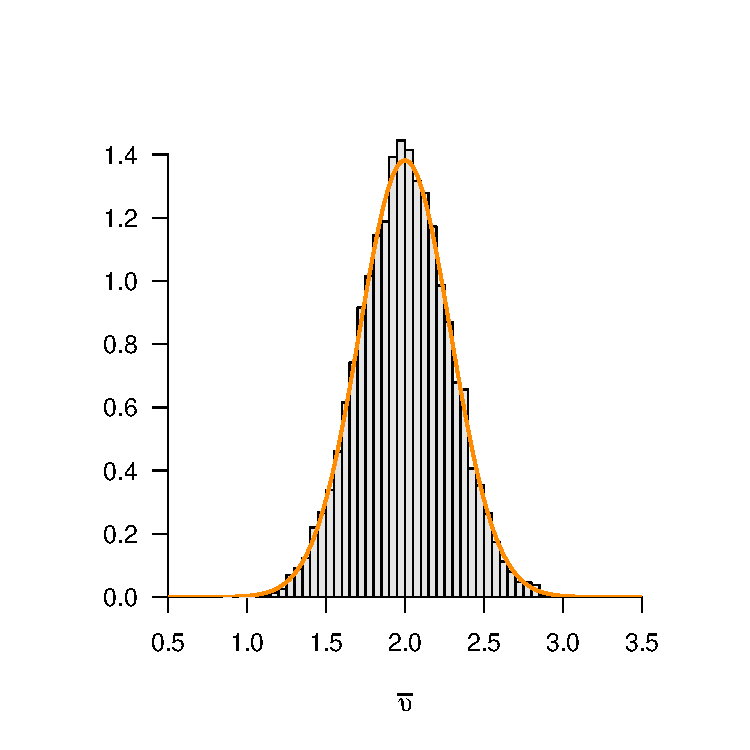
\includegraphics[width=0.5\linewidth]{6_Abbildungen/alm_6_beta_hat_1} \end{center}
\vfill
\end{frame}

\begin{frame}{Schätzerverteilungen}
\protect\hypertarget{schuxe4tzerverteilungen-1}{}
Beispiel (2) Einfache lineare Regression \vspace{1mm}

\small

Es sei \begin{equation}
\upsilon \sim N(X\beta, \sigma^2I_n) \mbox{ mit }
\begin{pmatrix}
1       & x_1       \\
\vdots  & \vdots    \\
1       & x_n
\end{pmatrix}
\in \mathbb{R}^{n\times 2},
\beta
\in \mathbb{R}^2,
\sigma^2 > 0.
\end{equation} das ALM Szenario der einfachen linearen Regression. Wir
haben bereits gesehen, dass \begin{equation}
\sigma^2(X^TX)^{-1}
=
\frac{\sigma^2}{s_x^2}
\begin{pmatrix}
  \frac{s_x^2}{n} + \bar{x}^2
& -\bar{x}
\\
  -\bar{x}
&  1
\end{pmatrix}
\mbox{ mit  }
s_x^2 := \sum_{i=1}^n (x_i - \bar{x})^2.
\end{equation} Die Varianz des Offsetparameterschätzers hängt also
sowohl von der Summe der quadrierten Differenzen und dem
Stichprobenmittel der unabhängigen Variablen \(x_1,...,x_n\) ab,
wohingegen die Varianz des Steigungsparameterschätzers nur von der Summe
der quadrierten Differenzen der \(x_1,...,x_n\) abhängt. Die Kovarianz
von Offset- und Steigungsparameterschätzern hängt vom Mittelwert der
\(x_1,...,x_n\) ab.
\end{frame}

\begin{frame}[fragile]{Schätzerverteilungen}
\protect\hypertarget{schuxe4tzerverteilungen-2}{}
Beispiel (2) Einfache lineare Regression \vspace{1mm} \setstretch{1.2}
\footnotesize

\begin{Shaded}
\begin{Highlighting}[]
\CommentTok{\# Modellformulierung}
\FunctionTok{library}\NormalTok{(MASS)                                         }\CommentTok{\# Multivariate Normalverteilung}
\NormalTok{n        }\OtherTok{=} \DecValTok{10}                                         \CommentTok{\# Anzahl von Datenpunkten}
\NormalTok{p        }\OtherTok{=} \DecValTok{2}                                          \CommentTok{\# Anzahl von Betparametern}
\NormalTok{x        }\OtherTok{=} \DecValTok{1}\SpecialCharTok{:}\NormalTok{n                                        }\CommentTok{\# Prädiktorwerte}
\NormalTok{X        }\OtherTok{=} \FunctionTok{matrix}\NormalTok{(}\FunctionTok{c}\NormalTok{(}\FunctionTok{rep}\NormalTok{(}\DecValTok{1}\NormalTok{,n),x), }\AttributeTok{nrow =}\NormalTok{ n)            }\CommentTok{\# Designmatrix}
\NormalTok{I\_n      }\OtherTok{=} \FunctionTok{diag}\NormalTok{(n)                                    }\CommentTok{\# n x n Einheitsmatrix}
\NormalTok{beta     }\OtherTok{=} \FunctionTok{matrix}\NormalTok{(}\FunctionTok{c}\NormalTok{(}\DecValTok{0}\NormalTok{,}\DecValTok{1}\NormalTok{), }\AttributeTok{nrow =}\NormalTok{ p)                   }\CommentTok{\# wahrer,aber unbekannter,Betaparameter}
\NormalTok{sigsqr   }\OtherTok{=}\NormalTok{ .}\DecValTok{5}                                         \CommentTok{\# wahrer,aber unbekannter,Varianzparameter}

\CommentTok{\# Frequentistische Simulation}
\NormalTok{nsim     }\OtherTok{=} \DecValTok{10}                                         \CommentTok{\# Anzahl Realisierungen n{-}dimensionaler ZV}
\NormalTok{y        }\OtherTok{=} \FunctionTok{matrix}\NormalTok{(}\FunctionTok{rep}\NormalTok{(}\ConstantTok{NaN}\NormalTok{,n}\SpecialCharTok{*}\NormalTok{nsim), }\AttributeTok{nrow =}\NormalTok{ n)          }\CommentTok{\# y Realisierungsarray}
\NormalTok{beta\_hat }\OtherTok{=} \FunctionTok{matrix}\NormalTok{(}\FunctionTok{rep}\NormalTok{(}\ConstantTok{NaN}\NormalTok{,p}\SpecialCharTok{*}\NormalTok{nsim), }\AttributeTok{nrow =}\NormalTok{ p)          }\CommentTok{\# \textbackslash{}hat\{\textbackslash{}beta\} Realisierungsarray}
\ControlFlowTok{for}\NormalTok{(i }\ControlFlowTok{in} \DecValTok{1}\SpecialCharTok{:}\NormalTok{nsim)\{}
\NormalTok{  y[,i]        }\OtherTok{=} \FunctionTok{mvrnorm}\NormalTok{(}\DecValTok{1}\NormalTok{, X }\SpecialCharTok{\%*\%}\NormalTok{ beta, sigsqr}\SpecialCharTok{*}\NormalTok{I\_n)   }\CommentTok{\# eine Realisierung n{-}dimensionaler ZV}
\NormalTok{  beta\_hat[,i] }\OtherTok{=} \FunctionTok{solve}\NormalTok{(}\FunctionTok{t}\NormalTok{(X) }\SpecialCharTok{\%*\%}\NormalTok{ X) }\SpecialCharTok{\%*\%} \FunctionTok{t}\NormalTok{(X) }\SpecialCharTok{\%*\%}\NormalTok{ y[,i] }\CommentTok{\# \textbackslash{}hat\{\textbackslash{}beta\} = (X\^{}T)X\^{}\{{-}1\}X\^{}T\textbackslash{}upsilon}
\NormalTok{\}}
\end{Highlighting}
\end{Shaded}
\end{frame}

\begin{frame}{Schätzerverteilungen}
\protect\hypertarget{schuxe4tzerverteilungen-3}{}
Beispiel (2) Einfache lineare Regression

\vspace{4mm}
\center

\(\quad\quad\quad\quad \upsilon \sim (X\beta,\sigma^2I_n)\) \hspace{3cm}
\(\hat{\beta} \sim N(\beta,\sigma^2(X^TX)^{-1})\)

\begin{center}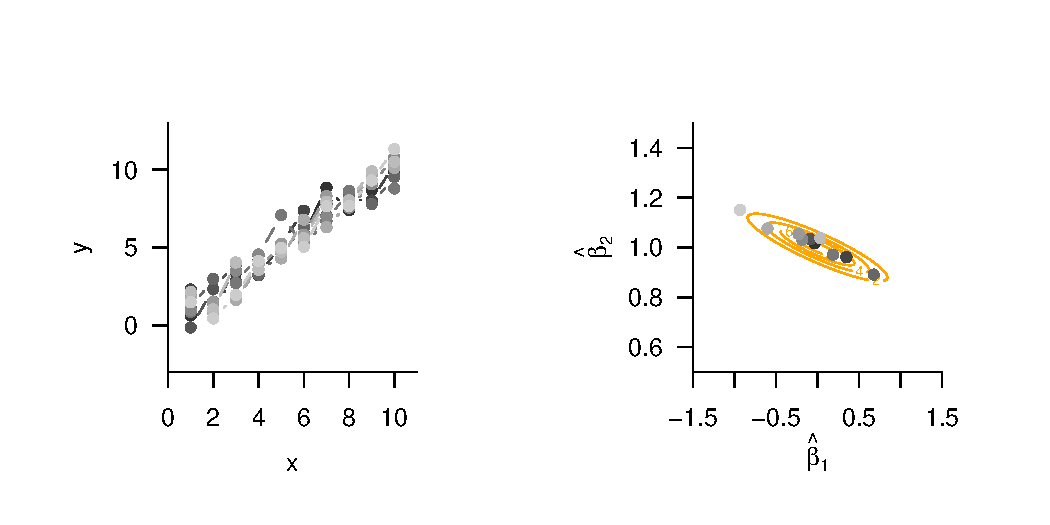
\includegraphics[width=1\linewidth]{6_Abbildungen/alm_6_beta_hat_2} \end{center}
\end{frame}

\begin{frame}{Schätzerverteilungen}
\protect\hypertarget{schuxe4tzerverteilungen-4}{}
\footnotesize
\begin{theorem}[Frequentistische Verteilung des Varianzparameterschätzers]
\normalfont
\justifying
Es sei
\begin{equation}
\upsilon = X\beta + \varepsilon \mbox{ mit } \varepsilon \sim N(0_n,\sigma^2I_n)
\end{equation}
das ALM. Weiterhin sei
\begin{equation}
\hat{\sigma}^2 = \frac{(\upsilon -  X\hat{\beta})^T(\upsilon -  X\hat{\beta})}{n-p}
\end{equation}
der Varianzparameterschätzer. Dann gilt
\begin{equation}
\frac{n-p}{\sigma^2}\hat{\sigma}^2 \sim \chi^2(n-p)
\end{equation}
\end{theorem}

Bemerkungen

\begin{itemize}
\tightlist
\item
  \justifying Wir verzichten auf einen Beweis. Da es sich bei
  \((\upsilon-X\hat{\beta})^T(\upsilon-X\hat{\beta})\) um eine Summe
  quadrierter normalverteilter Zufallsvariablen handelt, liegt die
  \(\chi^2\)-Verteilung im Lichte der \(\chi^2\) Transformation aus
  Einheit (8) Transformationen der Normalverteilung in
  Wahrscheinlichkeitstheorie und Frequentistische Inferenz zumindest
  nahe.
\end{itemize}
\end{frame}

\begin{frame}{Schätzerverteilungen}
\protect\hypertarget{schuxe4tzerverteilungen-5}{}
Beispiel (1) Unabhängige und identisch normalverteilte Zufallsvariablen
\vspace{1mm}

\small

Es sei \begin{equation}
\upsilon \sim N(X\beta,\sigma^2 I_n)
\mbox{ mit }
X := 1_n \in \mathbb{R}^{n\times 1},
\beta := \mu \in \mathbb{R}
\mbox{ und } \sigma^2 > 0.
\end{equation} das ALM Szenario unabhängiger und identisch
normalverteilter Zufallsvariablen. Wir haben bereits gesehen, dass in
diesem Fall \(\hat{\beta}\) mit dem Stichprobenmittel \(\bar{\upsilon}\)
identisch ist und dass \(\hat{\sigma}^2\) mit der Stichprobenvarianz
\(s^2_\upsilon\) übereinstimmt.

In Einheit (11) Konfidenzintervalle von Wahrscheinlichkeitstheorie und
Frequentistische Inferenz hatten wir für den Fall von \(n\) unabhängig
und identisch normalverteilten Zufallsvariablen die Statistik
\begin{equation}
U := \frac{n-1}{\sigma^2}S^2
\end{equation} definiert und festgehalten, dass \begin{equation}
U \sim \chi^2(n-1).
\end{equation} Offenbar ist \(U\) für \(p = 1\) mit der im obigen
Theorem betrachten Zufallsvariable
\(\frac{n-p}{\sigma^2}\hat{\sigma}^2\) identisch.
\end{frame}

\begin{frame}[fragile]{Schätzerverteilungen}
\protect\hypertarget{schuxe4tzerverteilungen-6}{}
Beispiel (2) Einfache lineare Regression \vspace{2mm} \tiny

\begin{Shaded}
\begin{Highlighting}[]
\CommentTok{\# Modellfumuliertung}
\FunctionTok{library}\NormalTok{(MASS)                                          }\CommentTok{\# multivariate Normalverteilung}
\NormalTok{n          }\OtherTok{=} \DecValTok{10}                                        \CommentTok{\# Anzahl von Datenpunkten}
\NormalTok{p          }\OtherTok{=} \DecValTok{2}                                         \CommentTok{\# Anzahl von Betparametern}
\NormalTok{x          }\OtherTok{=} \DecValTok{1}\SpecialCharTok{:}\NormalTok{n                                       }\CommentTok{\# Prädiktorwerte}
\NormalTok{X          }\OtherTok{=} \FunctionTok{matrix}\NormalTok{(}\FunctionTok{c}\NormalTok{(}\FunctionTok{rep}\NormalTok{(}\DecValTok{1}\NormalTok{,n),x), }\AttributeTok{nrow =}\NormalTok{ n)           }\CommentTok{\# Designmatrix}
\NormalTok{I\_n        }\OtherTok{=} \FunctionTok{diag}\NormalTok{(n)                                   }\CommentTok{\# n x n Einheitsmatrix}
\NormalTok{beta       }\OtherTok{=} \FunctionTok{matrix}\NormalTok{(}\FunctionTok{c}\NormalTok{(}\DecValTok{0}\NormalTok{,}\DecValTok{1}\NormalTok{), }\AttributeTok{nrow =}\NormalTok{ p)                  }\CommentTok{\# wahrer,aber unbekannter,Betaparameter}
\NormalTok{sigsqr     }\OtherTok{=}\NormalTok{ .}\DecValTok{5}                                        \CommentTok{\# wahrer,aber unbekannter,Varianzparameter}

\CommentTok{\# Frequentistische Simulation}
\NormalTok{nsim       }\OtherTok{=} \FloatTok{1e3}                                       \CommentTok{\# Anzahl Realisierungen n{-}dimensionaler ZV}
\NormalTok{y          }\OtherTok{=} \FunctionTok{matrix}\NormalTok{(}\FunctionTok{rep}\NormalTok{(}\ConstantTok{NaN}\NormalTok{,n}\SpecialCharTok{*}\NormalTok{nsim), }\AttributeTok{nrow =}\NormalTok{ n)         }\CommentTok{\# y Realisierungsarray}
\NormalTok{beta\_hat   }\OtherTok{=} \FunctionTok{matrix}\NormalTok{(}\FunctionTok{rep}\NormalTok{(}\ConstantTok{NaN}\NormalTok{,p}\SpecialCharTok{*}\NormalTok{nsim), }\AttributeTok{nrow =}\NormalTok{ p)         }\CommentTok{\# \textbackslash{}hat\{\textbackslash{}beta\} Realisierungsarray}
\NormalTok{sigsqr\_hat }\OtherTok{=} \FunctionTok{rep}\NormalTok{(}\ConstantTok{NaN}\NormalTok{, nsim)                            }\CommentTok{\# \textbackslash{}hat\{\textbackslash{}sigma\}\^{}2 Realisierungsarray}
\ControlFlowTok{for}\NormalTok{(i }\ControlFlowTok{in} \DecValTok{1}\SpecialCharTok{:}\NormalTok{nsim)\{}
\NormalTok{  y[,i]         }\OtherTok{=} \FunctionTok{mvrnorm}\NormalTok{(}\DecValTok{1}\NormalTok{, X }\SpecialCharTok{\%*\%}\NormalTok{ beta, sigsqr}\SpecialCharTok{*}\NormalTok{I\_n)   }\CommentTok{\# eine Realisierung n{-}dimensionaler ZV}
\NormalTok{  beta\_hat[,i]  }\OtherTok{=} \FunctionTok{solve}\NormalTok{(}\FunctionTok{t}\NormalTok{(X) }\SpecialCharTok{\%*\%}\NormalTok{ X) }\SpecialCharTok{\%*\%} \FunctionTok{t}\NormalTok{(X) }\SpecialCharTok{\%*\%}\NormalTok{ y[,i] }\CommentTok{\# \textbackslash{}hat\{\textbackslash{}beta\}    = (X\^{}T)X\^{}\{{-}1\}X\^{}T\textbackslash{}upsilon}
\NormalTok{  eps\_hat       }\OtherTok{=}\NormalTok{ y[,i] }\SpecialCharTok{{-}}\NormalTok{ X }\SpecialCharTok{\%*\%}\NormalTok{ beta\_hat[,i]           }\CommentTok{\# \textbackslash{}hat\{\textbackslash{}eps\}     = \textbackslash{}upsilon{-}X\textbackslash{}hat\{\textbackslash{}beta\}}
\NormalTok{  sigsqr\_hat[i] }\OtherTok{=}\NormalTok{ (}\FunctionTok{t}\NormalTok{(eps\_hat) }\SpecialCharTok{\%*\%}\NormalTok{ eps\_hat)}\SpecialCharTok{/}\NormalTok{(n}\SpecialCharTok{{-}}\NormalTok{p)       }\CommentTok{\# \textbackslash{}hat\{\textbackslash{}sigma\}\^{}2 =\textbackslash{}hat\{\textbackslash{}eps\}\^{}T\textbackslash{}hat\{\textbackslash{}eps\}/(n{-}p)}
\NormalTok{\}}
\NormalTok{U }\OtherTok{=}\NormalTok{ ((n}\SpecialCharTok{{-}}\NormalTok{p)}\SpecialCharTok{/}\NormalTok{sigsqr)}\SpecialCharTok{*}\NormalTok{sigsqr\_hat                          }\CommentTok{\# \textbackslash{}chi\^{}2 verteilte Zufallsvariable}
\end{Highlighting}
\end{Shaded}
\end{frame}

\begin{frame}{Schätzerverteilungen}
\protect\hypertarget{schuxe4tzerverteilungen-7}{}
Beispiel (2) Einfache lineare Regression

\vspace{4mm}
\center

\(\quad\quad \upsilon \sim (X\beta,\sigma^2I_n)\) \hspace{3cm}
\(\frac{n-p}{\sigma^2}\hat{\sigma}^2 \sim \chi^2(n-p)\)

\begin{center}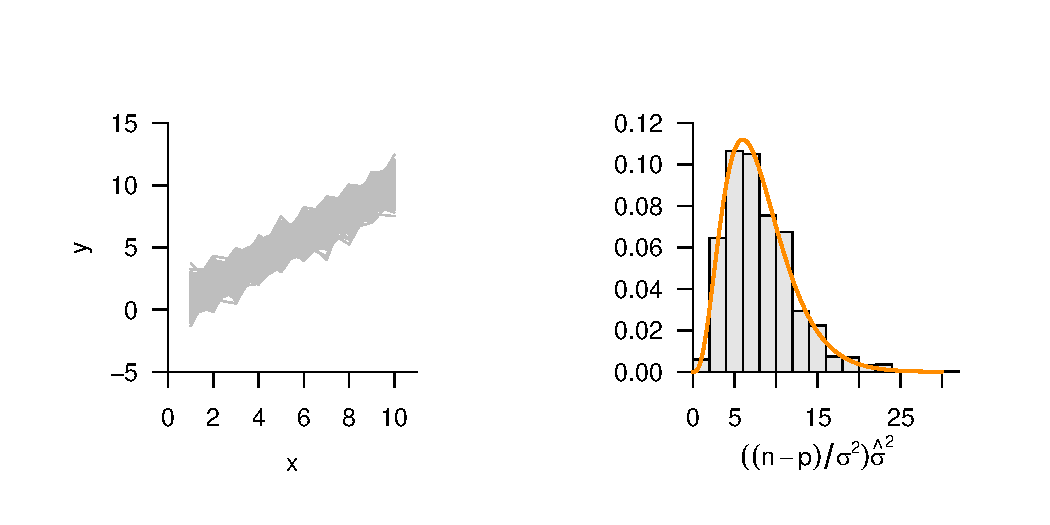
\includegraphics[width=1\linewidth]{6_Abbildungen/alm_6_sigsqr_hat_1} \end{center}
\end{frame}

\begin{frame}{}
\protect\hypertarget{section-12}{}
\large
\setstretch{2.7}
\vfill

Allgemeine Theorie

Unabhängige und identisch normalverteilte Zufallsvariablen

Einfache lineare Regression

Frequentistische Schätzerverteilungen

\textbf{Selbstkontrollfragen} \vfill
\end{frame}

\begin{frame}{Selbstkontrollfragen}
\protect\hypertarget{selbstkontrollfragen}{}
\footnotesize
\setstretch{3}

\begin{enumerate}
\tightlist
\item
  Geben Sie das Theorem zum Betaparameterschätzer wieder.
\item
  Warum ist der Betaparameterschätzer ein Maximum-Likelihood Schätzer?
\item
  Geben Sie das Theorem zum Varianzparameterschätzer wieder-
\item
  Geben Sie die Parameterschätzer bei \(n\) unabhängigen und identisch
  normalverteilten Zufallsvariablen an.
\item
  Geben Sie die Parameterschätzer bei einfacher linearer Regression an.
\item
  Geben Sie das Theorem zur Verteilung des Betaparameterschätzers
  wieder.
\item
  Geben Sie das Theorem zur Verteilung des Varianzparameterschätzers
  wieder.
\end{enumerate}
\end{frame}

\begin{frame}{Referenzen}
\protect\hypertarget{referenzen}{}
\footnotesize

\hypertarget{refs}{}
\begin{CSLReferences}{1}{0}
\leavevmode\vadjust pre{\hypertarget{ref-rencher_2008}{}}%
Rencher, Alvin C., and G. Bruce Schaalje. 2008. \emph{Linear Models in
Statistics}. 2nd ed. {Hoboken, N.J}: {Wiley-Interscience}.

\leavevmode\vadjust pre{\hypertarget{ref-searle_1971}{}}%
Searle, S. R. 1971. \emph{Linear Models}. A {Wiley} Publication in
Mathematical Statistics. {New York}: {Wiley}.

\end{CSLReferences}
\end{frame}

\end{document}
